%%%%%%%%%%%%%%%%%%%%%%%%%%%%%%%%%%%%%%%%%%%%%%%%%%%%%%%%%%%%%%%%%%%%%%%%%%%%%%%%
%%
%% Para utilizar ese modelo sao necessarios os seguintes arquivos:
%%
%% copin.cls
%% copin.sty
%% mestre.sty
%%
%%%%%%%%%%%%%%%%%%%%%%%%%%%%%%%%%%%%%%%%%%%%%%%%%%%%%%%%%%%%%%%%%%%%%%%%%%%%%%%%

\documentclass[a4paper,titlepage]{copin}
\usepackage[portuges,english]{babel}
\usepackage{copin,mestre,epsfig}
\usepackage{times}

%-------------------------- Para usar acentuacaoo em sistemas ISO8859-1 ------------------------------------
% Se estiver usando o Microsoft Windows ou linux com essa codificacao, descomente essa linhas abaixo
% e comente as linhas referentes ao UTF8
\usepackage[latin1]{inputenc} % Usar acentuacao em sistemas ISO8859-1, comentar a linha com  \usepackage[utf8x]{inputenc}
%-----------------------------------------------------------------------------------------------------

%-------------------------- Para usar acentuacao em sistemas UTF8 ------------------------------------
% Para a maior parte das distribuicoes linux, usar a opcao utf8x (lembrar de comentar as linha referente a ISO8859-1 acima)
\usepackage{ucs}
%\usepackage[utf8x]{inputenc}
%\usepackage[utf8]{inputenc}
\usepackage[T1]{fontenc}
%-----------------------------------------------------------------------------------------------------


\usepackage{fancyheadings}
\usepackage{graphicx}
\usepackage{caption}
\usepackage{subcaption}
\usepackage{longtable} %tabelas longas, para tabelas que ultrapassam uma pagina
%\input{psfig.sty}


% ----------------- Para inserir codigo fonte de linguagens de programacao no documento -------------
\usepackage{listings}
\lstset{numbers=left,
stepnumber=1,
firstnumber=1,
%numberstyle=\tiny,
extendedchars=true,
breaklines=true,
frame=tb,
basicstyle=\footnotesize,
stringstyle=\ttfamily,
showstringspaces=false
}
\renewcommand{\lstlistingname}{C\'odigo Fonte}
\renewcommand{\lstlistlistingname}{Lista de C\'odigos Fonte}
% ---------------------------------------------------------------------------------------------------

\selectlanguage{portuges}
\sloppy

\begin{document}

%%%%%%%%%%%%%%%%%%%%%%%%%%%%%%%%%%%%%%%%%%%%%%%%%%%%%%%%%%%%%%%%%%%%%%%%%%%%%%%%
\Titulo{Arcabou�o de Software para a Aquisi��o de Dados de Sa�de Atrav�s de Jogos Eletr�nicos}
\Autor{Ant�nio Dias dos Santos J�nior}
\Data{Fevereiro de 2013}
\Area{Ci�ncia da Computa��o}
\Pesquisa{Engenharia de Software}
\Orientadores{Angelo Perkusich (Orientador) \\
Hyggo Oliveira de Almeida (Orientador)}

\newpage
\cleardoublepage

\PaginadeRosto

\newpage
\cleardoublepage

%%%%%%%%%%%%%%%%%%%%%%%%%%%%%%%%%%%%%%%%%%%%%%%%%%%%%%%%%%%%%%%%%%%%%%%%%%%%%%%%
\begin{resumo} 
%A Doença de Parkinson (Parkinson) é uma doença neurodegenerativa que causa sintomas motores como: tremor de repouso, bradicinesia e anormalidade na marcha. A natureza progressiva da doença requer um monitoramento contínuo dos sintomas motores para auxiliar o neurologista no gerenciamento medicamentoso. Com este propósito, os Sistemas de Monitoramento da Saúde (SMS) são utilizados para prover esse cuidado com a saúde de forma descentralizada dos hospitais e ambientes clínicos. Todavia, a maioria dos pacientes rejeitam as soluções de SMS atuais, porque as consideram invasivas e estigmatizadas. Neste trabalho, é apresentado uma abordagem não-invasiva de SMS baseada em jogos eletrônicas voltada para o monioramento dos sintomas motores do Parkinson. Devido a natureza lúdica dos jogos eletrônicos, esta abordagem permite coletar dados dos pacientes sem relembrá-los que estão sob o tratamento da doença. Nós validamos esta abordagem junto a 30 sujeitos de pesquisa dividos em Grupo de Parkinson e Grupo Controle. A 
%aplicação dos dados numa Máquina de Vetor Suporte (SVM) identificou a ocorrência do sintoma motor da bradicinesia no Grupo de Parkinson obtendo uma acurácia de 86,66\%. Além disto, 90\% dos pacientes aprovaram a solução de SMS considerando-o não-invasivo e de fácil integração à rotina dos usuários.



Os Sistemas de Monitoramento da Saúde (SMS) podem melhorar a qualidade de vida dos usuários ao fornecer remotamente informações sobre o estado de saúde. Por outro lado, a concepção de um SMS dados motores não invasivo, ainda é um grande desafio multidisciplinar. Estes sistemas, apesar do avanço na tecnologia, ainda são visíveis e estereotipados, o que dificulta sua disseminação. Portanto, o uso destes sistemas não tem sido incorporado na rotina dos usuários, inviabilizando o monitoramento dos sintomas motores.
 
Diante da dificuldade de desenvolver um sistema com as características descritas, neste trabalho, propõe-se utilizar jogos eletrônicos para motivar e abstrair o monitoramento de dados de saúde. Estatísticas da indústria americana de jogos constataram que, em 2015, os jogadores de videogame possuíam em média 35 anos e, 27$\%$  estão acima dos 50 anos. Desde 2005, os jogos eletrônicos utilizam sensores de detecção de movimento para capturar as ações cinéticas do usuário. Desta forma, na abordagem proposta neste trabalho, o usuário executa movimentos específicos, em um jogo eletrônico para quantificar seus sinais motores e monitorar seu estado de saúde.

A relevância deste trabalho foi validada por meio de pesquisa qualitativa, na qual foi realizada uma entrevista semiestruturada junto a profissionais de saúde. Para a validação da abordagem, foi realizado um estudo analítico de caso-controle para detectar indivíduos diagnosticados com a Doença de Parkinson (Parkinson), utilizando sensores de captura de movimento em jogos eletrônicos. Buscou-se avaliar as possibilidades de aquisição de dados de saúde, baseada nas características de Cinemática Angular do Movimento Humano. Estes dados foram aplicados em uma Máquina de Vetor de Suporte (SVM) para classificação dos dados. Como resultado, foi obtida uma taxa de identificação com acurácia de 86,67\% e falsos positivos de 6,67\%. Desta forma, concluiu-se que a abordagem proposta permite desenvolver jogos eletrônicos que servem como uma forma não invasiva para monitorar dados motores.




\end{resumo}

\newpage
\cleardoublepage

%%%%%%%%%%%%%%%%%%%%%%%%%%%%%%%%%%%%%%%%%%%%%%%%%%%%%%%%%%%%%%%%%%%%%%%%%%%%%%%%
\begin{summary}
The use of Health Monitoring System (HMS) can improve the patients' quality life by allowing the physician to have access to information of patients' health status. This allows early identification of symptoms or identify the occurrence of health critical situations. However, the motor monitoring requires a motor evaluation of the the patient's motility through movement wich allows an motor assessment. This is a real challenge to design a noninvasive and engaged HMS into users' daily routine.
The proposed system architecture, allows a HMS to electronic games that uses motion detection sensors to acquire motor signals from the kinetic actions of the user. Thus, within the context of an electronic game, the user is induced to perform movements that assess their health status in a playful environment and away from the health care context. To evaluate this architecture, it was developed an electronic game using this architecture and held an analytical case-control study to detect individuals diagnosed with Parkinson's disease (Parkinson). So, in this experiment we quantified the motion characteristics using the angular kinects of the human movement, where the acquired data were applied to a Support Vector Machine (SVM) responsible to identify the occurrence of a Parkinson's motor symptom. In our results, we obtained a data classification accuracy of 86.67\% and false positive rate of 6.67\% Moreover, in users' acceptance evaluation, 90\% felt motivated with the developed game and 
aswered they would integrate this HMS into his daily routine. So, according this experiments, we system architecture allows the development of games with the monitoring purpose of the users' motor evaluation integrated into his daily routine.




%VERSÂO ANTERIOR
Health Monitoring Systems (HMS) can improve users' quality life by remotely providing information to remotely provide information about the health status, allowing early identification of critical situations. However, to monitor the users' motor health is necessary to perform clinical movements that allow the motor evaluation. For this reason, the design of a noninvasive SMS for motor health is still a multidisciplinary challenge.


However, the developemnt of a non-invasive health monitoring system for motor data is a multidisciplinary challenge. These systems, despite technology advancements, are still invasive and stereotyped, what makes difficult their dissemination. So, these systems have not been applied to the users daily activities, undermining motor symptoms monitoring.

This work proposes the use of video games to motivate and disregard health monitoring, integrating it in users daily routine. The proposed approach allows integrating the HMS architecture to electronic games that use motion detection sensors to capture users' kinetic actions. This way, the user performs specific movements inside the context of an electronic game that quantifies motion signals and monitors health.

To validate the approach, we performed a case-control analytic study to detect individuals diagnosed with Parkinson's Disease (PD) using motion capturing sensors through video games. We evaluated health data acquisition possibilities based on Human Motion Angular Kinetic characteristics. The data was applied in a Support Vector Machine (SVM) to classify the data. As a result, we had an accuracy rate of 86.67\% true positive identification and 6.67\% rate of false positive. This way, we concluded that the proposed approach allows developing video games to monitor motion data non-invasively.
\end{summary}

\newpage
\cleardoublepage

%%%%%%%%%%%%%%%%%%%%%%%%%%%%%%%%%%%%%%%%%%%%%%%%%%%%%%%%%%%%%%%%%%%%%%%%%%%%%%%%
\begin{agradecimentos}
Agrade�o aos meus pais e fam�lia, pois devo a eles tudo o que alcancei e me tornei.
� minha namorada, Mayelli, pela paci�ncia, cumplicidade e apoio incondicionais durante todo o tempo em que estivemos juntos. Obrigado por me entender nos momentos em que mais necessito e por estar sempre ao meu lado.
Aos amigos que fiz em Campina Grande, estudantes como eu, que dividiram comigo os momentos felizes e n�o t�o felizes da vida acad�mica. Agrade�o especialmente a Leonardo e Rafael, por sua contribui��o direta, indispens�vel para a realiza��o deste trabalho. Tamb�m a Romeryto e Maur�lio, grandes amigos e companheiros de sala.
�s funcion�rias da COPIN, por sua disposi��o a sempre ajudar n�s alunos da p�s-gradua��o.
Aos meus orientadores Angelo e Hyggo, por sua participa��o essencial neste trabalho, especialmente pela paci�ncia, aux�lio e id�ias valiosas.
� CAPES, pelo apoio financeiro.
\end{agradecimentos}

\clearpage

%%%%%%%%%%%%%%%%%%%%%%%%%%%%%%%%%%%%%%%%%%%%%%%%%%%%%%%%%%%%%%%%%%%%%%%%%%%%%%%%
%% Definicao do cabecalho: secao do lado esquerdo e numero da pagina do lado direito
\pagestyle{fancy}
\addtolength{\headwidth}{\marginparsep}\addtolength{\headwidth}{\marginparwidth}\headwidth = \textwidth
\renewcommand{\chaptermark}[1]{\markboth{#1}{}}
\renewcommand{\sectionmark}[1]{\markright{\thesection\ #1}}\lhead[\fancyplain{}{\bfseries\thepage}]%
	     {\fancyplain{}{\emph{\rightmark}}}\rhead[\fancyplain{}{\bfseries\leftmark}]%
             {\fancyplain{}{\bfseries\thepage}}\cfoot{}

%%%%%%%%%%%%%%%%%%%%%%%%%%%%%%%%%%%%%%%%%%%%%%%%%%%%%%%%%%%%%%%%%%%%%%%%%%%%%%%%
\selectlanguage{portuges}

\Sumario
%\ListadeSimbolos
\listoffigures
\listoftables
\lstlistoflistings %lista de codigos fonte - Para inserir a listagem de codigos fonte
\newpage
\cleardoublepage

\Introducao


%%%%%%%%%%%%%%%%%%%%%%%%%%%%%%%%%%%%%%%%%%%%%%%%%%%%%%%%%%%%%%%%%%%%%%%%%%%%%%%%
%
% Hifenizacao - Colocar lista de palavras que nao devem ser separadas e que 
% nao estao no dicionario portugues.
% As palavras do dicionario portugues ja sao separadas corretamente pelo lateX
%
\hyphenation{ Hardware Software etc  }

\chapter{Introdu\c{c}\~{a}o} \label{sec:intro}

Os gastos com sa�de totalizam 9\% do PIB no Brasil e 16,2\% nos Estados Unidos\footnote{https://www.cia.gov/library/publications/the-world-factbook/}. Os custos crescentes com assist�ncia � sa�de devido ao aumento na popula��o com mais de 60 anos nos pa�ses mostram a import�ncia de gerenciar recursos, focando no conforto do indiv�duo~\cite{Atallah2012}. Gra�as aos avan�os alcan�ados na �rea de tecnologia da informa��o e comunica��o, conceitos promissores como assist�ncia m�dica pervasiva (\emph{Pervasive Healthcare}) surgiram com potencial para auxiliar o atual sistema de assist�ncia � sa�de~\cite{varshney2009pervasive}. A assist�ncia m�dica pervasiva � um avan�o na assist�ncia � sa�de para qualquer pessoa, a qualquer hora e lugar, assistida por dispositivos computacionais integrados entre si e ao cotidiano das pessoas~\cite{Augusto:jucs_12_1}. Um desafio importante � prover essa qualidade de servi�os para um n�mero crescente de pessoas, otimizando o uso de recursos humanos e financeiros. O grande diferencial no uso de dispositivos inteligentes, interfaces com o usu�rio, sensores corporais e dispositivos de comunica��o sem fio dentro do contexto de assist�ncia m�dica consiste no monitoramento constante do estado de sa�de das pessoas, mesmo fora do hospital. Apesar desse monitoramento constante n�o ser capaz de eliminar completamente os erros m�dicos, existe um grande potencial de mitigar alguns dos problemas relacionados com a falta de informa��o~\cite{Varshney07}.

O monitoramento baseado em sensores que capturam dados de sa�de dos indiv�duos pode ser importante, por exemplo, para detec��o prematura de doen�as, ajudando tanto na preven��o destas quanto na administra��o de um melhor tratamento, podendo prover maior qualidade de vida para um indiv�duo. Formas de avalia��o da sa�de que podem ser realizadas atrav�s do monitoramento s�o sugeridas em~\cite{OgawaTogawa03}, como a determina��o do intervalo normal de cada dado capturado para cada indiv�duo, a an�lise estat�stica da correla��o entre os dados de sa�de e a predi��o de tend�ncias relativas � sa�de no futuro. Por fim, a an�lise dos dados capturados pode ajudar a identificar manifesta��es de sintomas que relacionam-se com a ocorr�ncia de um problema de sa�de, que podem ser vistos como um sinal prim�rio da doen�a, se ocorrerem repetidamente. A acumula��o de tais resultados dentro de uma popula��o pode ser usada n�o somente para diagnosticar mais cedo, mas tamb�m para identificar a origem da doen�a em estudos epidemiol�gicos.

Apesar de todas as vantagens mencionadas e utilidades atribu�das aos sistemas de monitoramento, existem alguns problemas a serem mencionados. Dentre eles est�o a dificuldade de uso e a falta de motiva��o dos usu�rios. Atualmente, dados de sa�de capturados durante o monitoramento, tais como press�o sangu�nea, frequ�ncia card�aca e temperatura, por exemplo, s�o sincronizados com um servidor externo para que sejam armazenados e/ou analisados por profissionais de sa�de~\cite{Gouaux2003,Motoi2009,Pantelopoulos2010}. Os sistemas pessoais de monitoramento de sa�de requerem que o usu�rio tenha disciplina durante a leitura dos seus dados de sa�de, ou que ao menos esteja utilizando os sensores corretamente para obter uma leitura satisfat�ria. Desta forma, os mecanismos de monitoramento tradicionais podem ser considerados entediantes pelas pessoas~\cite{Kato10}. Certos m�todos podem ser repetitivos e cansativos, exigindo que sensores sejam acoplados ao corpo, tornando complicada a obten��o da colabora��o ativa do indiv�duo durante seu monitoramento. H� tamb�m a resist�ncia de indiv�duos ao monitoramento realizado em casa~\cite{Aarhus2010}, uma vez que certos tipos de monitoramento realizados no lar requerem uma adapta��o do ambiente. � necess�ria uma forma que estimule os indiv�duos a incluir o monitoramento na sua rotina, tornando-os participantes mais ativos do seu pr�prio tratamento, tornando este mais motivador e efetivo.

Embora j� seja poss�vel e vi�vel a utiliza��o de dispositivos para monitorar os usu�rios, essa tarefa ainda n�o est� integrada ao seu cotidiano. Nesse contexto, jogos eletr�nicos v�m sendo fortemente utilizados como ferramenta motivadora. Com as novas possibilidades de intera��o trazidas pelas novas tecnologias usadas em jogos para captura de movimento, � poss�vel inserir elementos inovadores no projeto de jogos eletr�nicos. Dispositivos e sensores, como aceler�metros, girosc�pios, c�meras, tapetes, esteiras e sensores de press�o, s�o utilizados no contexto de jogos para criar novas formas de intera��o com o usu�rio~\cite{Staiano201117}.

� neste contexto de utiliza��o de jogos para viabilizar um monitoramento de sa�de de usu�rios de forma motivadora e efetiva que se insere este trabalho. A abordagem aqui proposta visa permitir a coleta de dados de sa�de de indiv�duos saud�veis utilizando jogos, de forma a antecipar cen�rios de doen�a ou de complica��es de sa�de atrav�s da identifica��o de anormalidades entre os dados coletados.

\section{Problem�tica}

A ideia de usar elementos de projeto de jogos, como recompensas, desafios e elementos gr�ficos, dentro de contextos diferentes para motivar e aumentar a atividade e reten��o de usu�rios rapidamente ganhou �nfase. Isso tem gerado intenso debate e tamb�m est� presente em in�meras aplica��es, como finan�as, sa�de e educa��o~\cite{Deterding2011}.

As aplica��es na sa�de que usam elementos de jogos s�o dirigidas a aumentar a motiva��o de indiv�duos em tr�s �reas. Primeiro, para aumentar o empenho de um indiv�duo em aprender mais sobre sua condi��o e tratamento. Segundo, para ser usado como uma ferramenta terap�utica de distra��o contra a dor e ansiedade. E, por fim, para encorajar indiv�duos jovens a continuar com longos tratamentos~\cite{Watters06}.

As primeiras aplica��es de jogos no contexto de sa�de ocorreram com o desenvolvimento de uma interface inovadora, de forma que jogos que tipicamente n�o exigiam nenhum esfor�o f�sico passaram a ser usados para motivar adultos e adolescentes a engajar-se em terapias e atividades f�sicas~\cite{Kato10}.

Os avan�os no desenvolvimento de interfaces alcan�ados pela ind�stria de jogos incluem tecnologias que fazem um rastreamento espacial, permitindo ao jogador controlar o ambiente do jogo com movimentos do seu corpo. As plataformas mais conhecidas atualmente s�o o Kinect, para o Xbox 360 da Microsoft; o Wii, da Nintendo; o EyeToy, usado no PlayStation2 da Sony, e o Move, para PlayStation3. As plataformas EyeToy e Kinect utilizam c�meras para capturar o movimento do jogador, enquanto que o Move e Wii utilizam uma combina��o de aceler�metros, girosc�pios e sensores infravermelho~\cite{Sandlund2011}. Na Figura~\ref{img:devices}, ilustra-se o Kinect, o controle do Wii e o PsMove.

\begin{figure}[!htb]
     \centering
     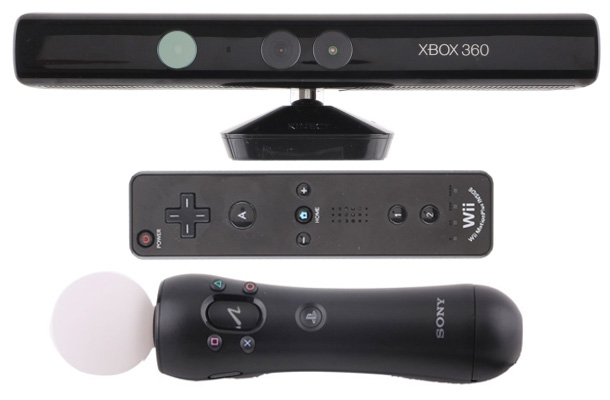
\includegraphics[width=0.7\textwidth]{motion-gaming-versus_610x400.jpg}
     \caption{Kinect, WiiMote e PsMove, de cima para baixo}
     \label{img:devices}
\end{figure}

Essas novas formas de intera��o com jogos digitais requerem naturalmente que o jogador seja mais ativo fisicamente durante o curso do jogo. Com essa inova��o surgiram os \emph{Exergames}~\cite{Staiano201117}, cujo nome � um termo criado a partir da combina��o de \emph{exercise} e \emph{digital gaming}, estimulando o jogador a empenhar-se no desenvolvimento de habilidades motoras durante o jogo. \emph{Exergames} foram primariamente projetados para promover o gasto cal�rico e elevar os batimentos card�acos atrav�s de atividade aer�bica, isto �, motivando a pr�tica de exerc�cios durante o curso de um jogo eletr�nico, uma vez que nem todos os indiv�duos t�m a motiva��o para praticar exerc�cios necess�rios para evitar a ocorr�ncia de doen�as ou diminuir sua progress�o. Dispositivos e sensores como aceler�metros, girosc�pios, c�meras, tapetes, esteiras e sensores de press�o s�o utilizados no contexto de exergames para medir a intera��o com o usu�rio. Alguns dos exergames comerciais mais conhecidos s�o o Dance Dance Revolution e o Wii Fit. Apesar de esses jogos n�o serem destinados primariamente � melhoria da sa�de, foram constatados efeitos positivos do seu uso~\cite{Assad2011,Jimison2008}.

Alguns jogos que se inserem no contexto de sa�de s�o classificados como jogos de diagn�stico m�dico, que s�o jogos usados para examinar um indiv�duo sob a suspeita de que j� possuem algum problema de sa�de. Para jogos de diagn�stico funcionarem corretamente, t�cnicas e pesquisas adequadas devem ser aplicadas ao mecanismo central do jogo para diagnosticar o indiv�duo com precis�o. Uma das quest�es mais importantes a se tratar em jogos para diagn�stico � manter a coleta de dados discreta e o n�vel de estresse do indiv�duo baixo. Um indiv�duo que est� ansioso e sob press�o por estar sendo submetido a v�rios exames pode n�o prover resultados precisos e, portanto, os tratamentos seguintes podem n�o ser t�o efetivos. Por isso, jogos para diagn�stico devem ser mantidos em um n�vel casual, para que fa�am o indiv�duo sentir-se como se n�o estivesse sendo examinado~\cite{Atkinson2010}.

Para que aplica��es direcionadas ao monitoramento da sa�de sejam poss�veis, a aquisi��o de dados dos jogadores pode ser feita com o uso de sensores e dispositivos de entrada diversos, como, por exemplo, um controle que capte movimentos atrav�s de aceler�metros. As novas possibilidades de intera��o desenvolvidas pela ind�stria de jogos v�o al�m dos m�todos convencionais de entrada, podendo ser usadas para avaliar as capacidades motoras e cognitivas de um jogador~\cite{Assad2011}.

O problema � que as abordagens j� propostas de jogos para a sa�de t�m como objetivo principal a execu��o de exerc�cios espec�ficos. Neste caso, o indiv�duo ainda se sente em tratamento ou sob monitoramento, podendo apresentar a mesma resist�ncia que existe no caso do monitoramento tradicional. Os jogos desenvolvidos para exerc�cios, reabilita��o e recupera��o envolvem movimentos repetitivos que podem deixar de ser atrativos para os usu�rios ap�s algum tempo de jogo. Ainda que o indiv�duo esteja jogando para seu pr�prio benef�cio, o jogo deve possuir fatores que incitem sua motiva��o para continuar jogando, como o n�vel de dificuldade, enredo, conex�o com o jogador e n�vel de engajamento~\cite{Watters06,Assad2011,Hardy11}. Al�m disso, algumas abordagens que utilizam jogos para monitoramento n�o levam em conta o fator idade~\cite{Atkinson2010}. Adolescentes e adultos jovens s�o um grupo de idade considerado complicado de obter participa��o ativa durante um tratamento~\cite{Kato10}. Apesar de jogos serem indicados para prover motiva��o, eles perdem sua atratividade para a faixa et�ria � qual esse tipo de abordagem � direcionada.

O problema de falta de motiva��o � ainda mais evidente quando se fala no monitoramento de indiv�duos saud�veis, que n�o t�m como motiva��o direta o tratamento de uma doen�a j� existente. Para estas pessoas, a atratividade do jogo em si � o �nico motivo pelo qual elas iriam utilizar o mesmo. Em resumo, enuncia-se o seguinte problema de pesquisa: como viabilizar o monitoramento de sa�de de indiv�duos utilizando jogos ainda mantendo a atratividade dos mesmos?

\section{Objetivo}

Neste trabalho, tem-se como objetivo desenvolver um arcabou�o de software para tratar a aquisi��o de dados de diferentes sensores e dispositivos de entrada utilizados em jogos eletr�nicos para posterior convers�o destes dados em informa��o sobre a sa�de do usu�rio. O arcabou�o define componentes de software que encapsulam regras para a tradu��o dos dados do usu�rio em informa��o sobre a sa�de. As regras definidas pelos componentes especificam informa��es sobre sintomas e caracter�sticas espec�ficas, e classificam os dados capturados atrav�s da intera��o com os jogos, transformando-os em informa��o de sa�de sobre o usu�rio.

Para permitir que os dados de sa�de de um indiv�duo sejam coletados durante o jogo de forma impercept�vel para o indiv�duo, a aquisi��o de dados deve ser feita por sensores e outros dispositivos de entrada de forma integrada com o enredo do pr�prio jogo. Os dados capturados s�o transmitidos para um componente do arcabou�o, que os armazena e, posteriormente, os trata. Dessa forma, os eventuais movimentos espec�ficos realizados pelo usu�rio que caracterizam defici�ncias psicomotoras, tais como tremores, dificuldades ou anomalias nos movimentos, ser�o registrados durante o curso do jogo, montando um hist�rico de sa�de. Este hist�rico pode ser utilizado no futuro, por exemplo, para identificar o in�cio de alguma defici�ncia de movimentos do indiv�duo.

O arcabou�o proposto possibilita a inser��o de mecanismos de captura de dados de sa�de a um jogo em tempo de desenvolvimento. Atrav�s de mecanismos bem definidos, s�o inseridos elementos no projeto do jogo que permitem que a captura de dados de sa�de seja integrada de forma transparente ao seu fluxo. Esses elementos podem ser, movimentos espec�ficos requeridos do jogador para controlar o jogo, ou um enredo e cen�rio adaptados para captar determinados dados em situa��es espec�ficas, como, por exemplo, falar uma palavra espec�fica para realizar an�lise de voz.

A hip�tese � que jogos eletr�nicos comuns, n�o direcionados para a sa�de, continuam sendo atrativos ao suprirem a falta de motiva��o enfrentada pelos sistemas de monitoramento convencionais, tornando mais f�cil a aquisi��o dos dados dos indiv�duos durante o curso do jogo. Ao inserir mecanismos de aquisi��o de dados em g�neros de jogos comuns, tem-se uma maior possibilidade de aceita��o do indiv�duo, por n�o existir a press�o psicol�gica de estar sendo monitorado.

Com o objetivo de realizar a valida��o, foram desenvolvidos dois jogos em parceria com o Instituto Federal de Alagoas (IFAL) utilizando a abordagem proposta para capturar os dados. Um dos jogos � o \emph{Pinball World}, que utiliza o aceler�metro de um dispositivo Android para controlar uma esfera atrav�s de um labirinto. O jogo captura os dados de tremor do usu�rio durante o curso do jogo. O segundo jogo, o \emph{Catch the Spheres}, capta dados de movimentos do corpo atrav�s do Kinect, testando o reflexo e velocidade de movimento do jogador ao capturar bolas que v�m em sua dire��o. Um experimento para demonstrar o funcionamento do arcabou�o foi realizado. Dezoito pessoas foram selecionadas para jogar e solicitadas a responder um question�rio sobre suas percep��es em rela��o ao jogo. Os resultados indicam que � poss�vel utilizar jogos casuais para o monitoramento. Os jogos desenvolvidos foram considerados divertidos e de f�cil entendimento pela maioria (61\%) dos participantes do experimento. Eles tamb�m declararam que incluiriam jogos casuais, n�o direcionados para monitoramento da sa�de, em sua rotina di�ria. Parte do experimento realizado consistiu em pedir para os participants simularem um movimento mais lento durante o jogo. Foi poss�vel detectar uma redu��o na velocidade de movimento de alguns participantes, quando lhes foi pedido para capturarem as bolas mais lentamente no jogo \emph{Catch the Spheres}. N�o foi detectado um n�vel de tremor significativo atrav�s do jogo \emph{Pinball World}.

\section{Relev�ncia}

Sabe-se que existem vantagens em descobrir os primeiros sinais de condi��es adversas de sa�de mais cedo, como redu��o de custos com sa�de e a redu��o de riscos relacionados a doen�as debilitantes~\cite{Kiss2011}. Para prover um tratamento mais eficaz, os primeiros sinais que caracterizam a manifesta��o de uma doen�a precisam ser detectados antes que sintomas maiores apare�am~\cite{OgawaTogawa03}. Uma das formas de detectar sinais prim�rios de uma condi��o de sa�de � o monitoramento.

Existe a necessidade de uma abordagem de avalia��o do indiv�duo que auxilie o m�dico na aplica��o do seu conhecimento e que diminua a depend�ncia de informa��es providas pelo indiv�duo. Se os dados necess�rios para a avalia��o forem capturados automaticamente, pode-se aumentar a qualidade da informa��o capturada, atrav�s coleta de dados de sa�de integrada � rotina do indiv�duo, e reduzir a carga de trabalho dos profissionais de sa�de que dela necessitam. Capturar dados de sa�de durante uma atividade prazerosa para o indiv�duo como um jogo interativo � uma forma de monitoramento diferente das tradicionais, que torna o indiv�duo mais propenso a contribuir com o seu monitoramento.

A principal contribui��o deste trabalho � a disponibiliza��o de um arcabou�o para desenvolvimento e an�lise de dados direcionados para o monitoramento da sa�de. No contexto de computa��o pervasiva, o arcabou�o prov� uma grande contribui��o por permitir o monitoramento de diversos par�metros de forma integrada � rotina do indiv�duo. O desenvolvimento de jogos para monitoramento de dados de sa�de e a an�lise dos dados obtidos s�o facilmente acess�veis para o desenvolvedor. O �nico passo necess�rio pro parte do desenvolvedor � escrever os dados coletados em um formato espec�fico, para ter acesso a m�dulos e m�todos de an�lise de dados providos pelo arcabou�o.

Este trabalho avan�a o estado da arte das solu��es de monitoramento n�o invasivo, contribuindo com atuais pesquisas dentro do laborat�rio Embedded, da Universidade Federal de Campina Grande, e tamb�m serve como base para futuras pesquisas na �rea de \emph{Pervasive Healthcare}.

\section{Organiza��o}

Este documento est� estruturado da seguinte forma. No Cap�tulo~\ref{cap:fundamentacao}, apresenta-se a fundamenta��o te�rica, onde
s�o apresentados os principais conceitos citados durante o trabaho, disponibilizando embasamento te�rico para os leitores. No Cap�tulo~\ref{cap:trabalhos}, s�o apresentados os principais trabalhos realizados no dom�nio de monitoramento atrav�s de jogos. No Cap�tulo~\ref{cap:arquitetura}, apresenta-se o Arcabou�o de Software para a Aquisi��o de Dados de Sa�de Atrav�s de Jogos Eletr�nicos. No Cap�tulo~\ref{cap:estudo}, s�o apresentados os dois estudos de caso constru�dos para validar o arcabou�o. E, finalmente, no Cap�tulo~\ref{cap:conclusao} apresenta-se a conclus�o do trabalho.
\chapter{Fundamenta��o Te�rica} \label{cap:fundamentacao}

\section{Assist�ncia M�dica Pervasiva (\emph{Pervasive Healthcare})}

O potencial da computa��o pervasiva pode ser percebido em v�rias perspectivas e ambientes, como hospitais, situa��es de emerg�ncia, na ind�stria, educa��o, entre outros. O termo Assist�ncia M�dica Pervasiva, ou \textit{Pervasive Healthcare}, � utilizado para descrever a integra��o da computa��o pervasiva na assist�ncia m�dica. A necessidade de sistemas de assist�ncia m�dica se deve ao fato de que profissionais da sa�de precisam de mobilidade, al�m de terem que compartilhar suas experi�ncias e informa��es com os demais profissionais respons�veis por determinado paciente~\cite{Varshney07,ahamed2007towards}.

A assist�ncia m�dica pervasiva � uma mudan�a de paradigma que, com o suporte apropriado, pode tornar as pessoas participantes ativas de seu pr�prio cuidado m�dico, prevenindo complica��es e reduzindo o avan�o da deteriora��o de suas condi��es. Para pacientes de alto risco, o cuidado proativo de profissionais de sa�de seguindo protocolos, planos e objetivos requer o uso de uma estrutura de tecnologias de comunica��o e informa��o, por exemplo, prontu�rios eletr�nicos compartilhados. A assist�ncia m�dica pervasiva usa a infraestrutura de tecnologias de comunica��o e informa��o para prover suporte a um estilo de vida assistido e independente, mantendo as pessoas em seu ambiente por tanto tempo quanto poss�vel, evitando a necessidade de serem internados~\cite{Augusto:jucs_12_1}.

Dentre os benef�cios do uso da assist�ncia pervasiva � sa�de tem-se: a melhoria do tratamento domiciliar do paciente~\cite{Aarhus2010}, a realiza��o do monitoramento remoto e monitoramento cont�nuo em pacientes que possuem n�veis cognitivos e f�sicos comprometidos~\cite{baker2007wireless}. Entretanto, a concep��o de um sistema de monitoramento cont�nuo e que n�o seja invasivo ainda � um grande desafio~\cite{Alemdar2010}. A necessidade de integrar diferentes sensores em uma �nica solu��o torna essa atividade mais dif�cil, devido a dispositivos pesados, vis�veis e estereotipados, como um sensor de ECG, por exemplo. Por esse motivo esses dispositivos enfrentam resist�ncia por parte dos usu�rios, que passam a n�o utiliz�-los no dia a dia, perdendo a possibilidade de monitoramento cont�nuo da sa�de~\cite{Aarhus2010,Alemdar2010}.

\section{Jogos S�rios}

Jogos s�rios s�o jogos que foram projetados especificamente para treinamento e educa��o. A maioria das pessoas pensa em jogos como uma forma de entretenimento. Entretanto, h� um interesse crescente em usar jogos para educar e treinar pessoas~\cite{annetta2010s}.

Apesar de existirem muitas defini��es para o termo, � consenso entre diferentes autores que o termo refere-se ao uso de jogos de computador cujo o principal prop�sito n�o � puramente entreter. De fato, jogos s�rios t�m sido aplicados em diversas �reas, como treinamento corporativo, cultural e militar, sa�de e educa��o. Muitas dessas �reas est�o relacionadas e se sobrep�em, como \textit{e-learning} (educa��o atrav�s de meios eletr�nicos), \textit{edutainment} (entretenimento com prop�stitos educativos) e aprendizado baseado em jogos comuns e digitais~\cite{rego2010serious}. O campo da medicina tem uma hist�ria de utiliza��o de jogos como meios de engajar os pacientes de forma comportamental para melhorar os resultados na sua sa�de. H� relat�rios antigos de estudos de caso usando jogos com pacientes passando por doen�as ou defici�ncias f�sicas~\cite{Kato10}.

Watters et al.~\cite{Watters06} afirmam que jogos para a sa�de s�o direcionados a aumentar a motiva��o de pacientes em tr�s �reas. Primeiro, aumentar a motiva��o do paciente para aprender mais sobre sua condi��o e seu tratamento. Segundo, para ser usado como uma ferramenta em uma terapia de distra��o para dor e ansiedade. E, por �ltimo, para encorajar pacientes jovens a continuarem com seus tratamentos prolongados. Nesta �ltima categoria, os jogos agem como "treinadores". Quando usados por crian�as, eles podem ajudar refor�ando as informa��es sobre o tratamento passadas na fase inicial, provendo um sistema de lembrete, encorajando a pr�tica de habilidades e gravando dados do tratamento e estado do usu�rio.

\section{\emph{Exergames}}

\emph{Exergame} � um termo formado a partir da combina��o de \textit{exercise} e \textit{digital gaming}. � uma pr�tica de exerc�cios f�sicos atrav�s de jogos eletr�nicos~\cite{sinclair2007considerations}. Esse tipo de jogo envolve o jogador em atividades que o permitem exercitar-se para desenvolver habilidades motoras durante o jogo, focando em grupos musculares maiores em vez de destreza manual ou capacidades motoras finas~\cite{Staiano201117}. Esse novo paradigma de entretenimento possibilitou � ind�stria de jogos criar t�tulos para favorecer a pratica de exerc�cios f�sicos, visando melhorar o condicionamento f�sico dos usuarios~\cite{suhonen2008seriously,gobel2010serious}. Atualmente existem trabalhos na �rea de fisioterapia verificando a efic�cia desses jogos para condicionamento f�sico, reabilita��o e aprendizagem motora para pessoas com problemas de mobilidade.

Apesar dos \emph{exergames} terem se tornado populares recentementes, a ideia de combinar movimento f�sico e seu reconhecimento atrav�s de vis�o computacional ou outra tecnologia sensorial n�o � inteiramente nova. Em 1982, o Atari Puffer\footnote{http://kotaku.com/5009577/atari-puffer-the-wii-fit-of-1982} foi desenvolvido, mas n�o lan�ado, como o primeiro \emph{exergame} usando uma bicicleta ergom�trica para controlar jogos no Atari 2600.

Nos �ltimos anos, a tend�ncia de \emph{exergames} comerciais n�o � somente usar os videogames como instrumento motivacional para encorajar a pr�tica de exerc�cios, mas tamb�m combin�-los com a coleta de par�metros vitais. Um exemplo proeminente disso � o \textit{EA Sports Active}, que tem como objetivo n�o somente reconhecer atividades via aceler�metros e medir a pulsa��o para prop�sitos relacionados � sa�de (telemonitoramento e an�lise de dados de exerc�cios), mas tamb�m melhorar o treinamento e resultados do uso de \textit{exergames} em geral~\cite{gobel2010serious}.

Os jogos \textit{Wii Sports} (2006) e \textit{Wii Fit} (2008) (Figura~\ref{img:wii_games}), produzidos pela Nintendo, s�o combina��es de jogos e pr�tica de exerc�cios, o que os insere na categoria de \emph{exergames}. Medindo pela popularidade dos jogos, pode-se simplesmente classific�-los como jogos unicamente l�dicos. A diferen�a � que o Wii Sports foca mais em ser um jogo l�dico, mas o Wii Fit tamb�m tem como objetivo ensinar algo sobre pr�tica de exerc�cios. O principal fator de efeito dos exerc�cios no Wii Sports � que ele utiliza controladores com sensores de movimento, como o Wii Remote (Wiimote) e o Nunchuk, que for�a o jogador a mover-se fisicamente quando est� jogando. O Nunchuk � uma extens�o que pode ser conectada ao Wiimote para possibilitar o controle de jogos com as duas m�os. No Wii Fit, uma balan�a tamb�m � utilizada durante o jogo~\cite{suhonen2009health}.

\begin{figure}[!htb]
     \centering
     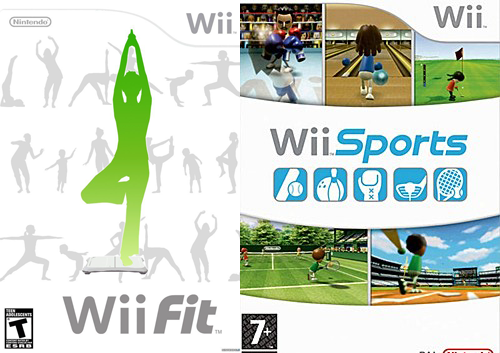
\includegraphics[width=.5\textwidth]{Wii_games.png}
     \caption{Os jogos Wii Fit e Wii Sports}
     \label{img:wii_games}
\end{figure}

\section{Sensores para Captura de Dados de Sa�de}

Atrav�s de determinados sensores para captura de dados de sa�de, � poss�vel capturar uma ou mais caracter�sticas que podem auxiliar no diagn�stico e monitoramento de doen�as. Redes de sensores montadas no lar podem ajudar pessoas e seus cuidadores, provendo monitoramento m�dico cont�nuo, controle de aparelhos dom�sticos, acesso a dados m�dicos e comunica��o de emerg�ncia. O monitoramento do estado de sa�de das pessoas � o tipo de aplica��o mais estudado em sistemas de assist�ncia m�dica pervasiva. Os sinais vitais mais utilizados s�o eletrocardiograma (ECG), oximetria de pulso, temperatura corporal, batimentos card�acos e press�o sangu�nea. Os dados de acelera��o tamb�m s�o utilizados com esses sinais vitais em alguns estudos~\cite{Alemdar2010}. No contexto de jogos, a utiliza��o de alguns sensores � impratic�vel, devido a seu tamanho, peso e forma de utilizar. Entretanto, sensores como c�meras~\cite{stach2009classifying,Sandlund2011}, aceler�metros e girosc�pios\cite{Staiano201117}, medidor de pulsa��o~\cite{masuko2006fitness} e Interfaces C�rebro-Computador~\cite{sherstyuk2010toward} v�m sendo utilizados com sucesso em jogos:

\begin{itemize}
  \item \textbf{Aceler�metros e girosc�pios:} um t�pico aceler�metro com seis graus de liberdade detecta acelera��o em tr�s eixos espaciais e a rota��o ao redor desses eixos. Aceler�metros s�o usados no Wiimote e Nunchuck da Nintendo e em outros tipos de jogos para detectar e interpretar diferentes tipos de movimento. A acur�cia do Nintendo Wii Motion Plus � melhorada utilizando girosc�pios.
  \item \textbf{C�meras:} podem ser usadas para capturar as posi��es e movimentos dos jogadores. Sistemas de vis�o b�sicos incluem o Sony EyeToy e o PlayStation Eye. V�rios jogos acad�micos usam uma ou mais c�meras para capturar o movimento do jogador. Uma abordagem relacionada � utilizar uma c�mera para rastrear marca��es infravermelhas. A vis�o computacional pode ser aumentada com outras tecnologias para melhorar sua acur�cia, como, por exemplo, um sensor de profundidade utilizado para produzir umagens 3D no Kinect, da Microsoft.
  \item \textbf{Medidores de pulsa��o:} s�o usados para promover a execu��o eficiente de atividades f�sicas, ajustando a intensidade dos exerc�cios baseado nos batimentos card�acos. O grau de dificuldade precisa ser ajustado efetivamente, para que os exerc�cios n�o se tornem mon�tonos.
  \item \textbf{Interfaces C�rebro-Computador:} l�em e analizam a atividade cerebral do jogador em tempo real. Os dois principais hardwares dispon�veis no mercado s�o o Emotiv Epoc\footnote{http://www.emotiv.com} e o MindSet, da NeuroSky\footnote{http://www.neurosky.com}. Os dispositivos traduzem diretamente as inten��es do jogador em a��es dentro do jogo, dispensando dispositivos como mouse, teclado ou joystick.
\end{itemize}

\chapter{Trabalhos Relacionados} \label{cap:trabalhos}

Apesar de se pensar em jogos apenas como uma forma de entretenimento, existe um interesse crescente em utiliz�-los para outras finalidades, devido a seu car�ter l�dico. Jogos eletr�nicos t�m sido usados para v�rios prop�sitos. No �mbito educacional, os jogos ajudam os estudantes no seu aprendizado, provendo uma forma diferente, motivadora e eficiente de absorver conte�do. Simuladores, que tamb�m podem ser encaixados na defini��o de jogos educacionais, oferecem uma alternativa vi�vel para o treinamento de pessoas. No campo de assist�ncia � sa�de, existem jogos comerciais que t�m o prop�sito de atingir certos objetivos comportamentais~\cite{Kato10}. Al�m dos prop�sitos j� mencionados, muitos trabalhos tratam sobre jogos que cuidam da motiva��o de pacientes para fazer exerc�cios e reabilita��o de pacientes com defici�ncias motoras.

\section{Video Games in Health Care: Closing the Gap}

Kato~\cite{Kato10} apresenta outros efeitos positivos de \emph{video games}, especialmente aqueles com foco em assist�ncia � sa�de. Segundo a autora, seres humanos nem sempre se comportam de forma a tomar vantagem do que a assist�ncia � sa�de tem a oferecer. A maioria das pessoas n�o age em conformidade com as condi��es que podem salvar suas vidas. As solu��es para esse problema s�o claramente complexas, mas os fatores psicol�gicos e comportamentais t�m um papel fundamental nessas solu��es. Neste sentido, jogos v�m sendo utilizados cada vez mais para endere�ar as barreiras psicol�gicas e comportamentais para a assist�ncia � sa�de �tima.

O mecanismo de a��o principal dos jogos geralmente citado � sua capacidade de aumentar a motiva��o. O foco da aten��o em uma distra��o provida por um jogo � visto como um fator fundamental para explicar como indiv�duos usam jogos para lidar com sintomas adversos, comportamentos dolorosos, adversos e entediantes.

\section{Adaptive Virtual Reality Games for Rehabilitation of Motor Disorders}

Ma et al.~\cite{Ma07} apresenta um sistema de treinamento para encorajar pacientes a praticarem exerc�cios f�sicos. O trabalho apresenta diretrizes �teis para a constru��o de um arcabou�o para jogos interativos direcionados � sa�de. Um dos fatores citados, que deve ser levado em conta na defini��o de um arcabou�o, � a constru��o de um perfil do paciente. De acordo com os autores, um fisioterapeuta geralmente criar� exerc�cios de terapia motora para um paciente baseado em um n�mero de fatores como: idade, sexo, hist�rico cultural, m�o com que escreve e condi��o m�dica (por exemplo, tempo desde o �ltimo derrame, hemiplegia do lado direito ou esquerdo e habilidades cognitivas, sensoriais e motoras, baseadas em testes padronizados).

Utilizando os dados do perfil e tamb�m alguma informa��o de contexto, n�o somente o n�vel de dificuldade dos exerc�cios, como tamb�m as partes do corpo ativas durante a tarefa poder�o ser adaptadas �s necessidades do paciente. As tarefas podem ser desenvolvidas para treinar um movimento espec�fico, como extens�o do punho, para aumentar a extens�o do movimento ou a resist�ncia da junta do punho.

A parte do sistema que trata da adapta��o din�mica usa os dados do perfil do paciente e os dados de seu progresso para selecionar atividades e configurar o n�vel de dificuldade das tarefas e do jogo. Assim, o sistema pode prover dados sobre o progresso individual dos pacientes, que podem ser comparados durante o per�odo de recupera��o para montar uma base de dados hist�rica do progresso do paciente. Um m�dulo de an�lise de dados possibilita a visualiza��o das trajet�rias de movimento dos pacientes e mostra os �ngulos das juntas, extens�o dos movimentos e velocidades.

Na Figura~\ref{img:ma_et_al}, ilustra-se a arquitetura do sistema. A entrada do ambiente de realidade virtual para treinamento se d� atrav�s de mouse e teclado para operadores do sistema, e dispositivos de captura de movimento em tempo real: duas luvas \emph{5DT Ultra DataGloves}\footnote{http://www.5dt.com/products/pdataglove5u.html} (Figura~\ref{fig:ultra}), al�m de quatro sensores magn�ticos sem-fio \emph{Ascension MotionStar}\footnote{http://www.ascension-tech.com/realtime/RTMotionSTARTethered.php} (Figura~\ref{fig:ams}), que s�o usados para captar movimentos das m�os, bra�os e parte superior do corpo. A sa�da envolve modalidades visuais, sonoras e h�pticas. A interface de sa�da visual inclui um monitor paraoperadores um dispositivo com visor montado sobre a cabe�a (\textit{Head Mounted Display} - HMD) de alta resolu��o (Figura~\ref{fig:hmd}).

\begin{figure}[!htb]
     \centering
     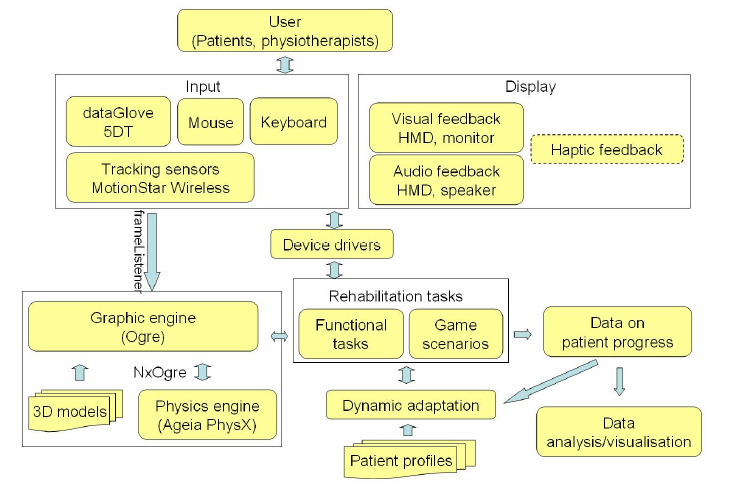
\includegraphics[width=1\textwidth]{ma_et_al.png}
     \caption{Arquitetura do sistema de realidade virtual para reabilita��o f�sica~\protect\cite{Ma07}}
     \label{img:ma_et_al}
\end{figure}

\begin{figure}
        \centering
        \begin{subfigure}[b]{0.3\textwidth}
                \centering
                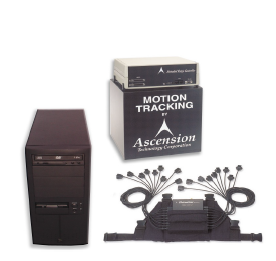
\includegraphics[width=\textwidth]{motionstar.png}
                \caption{Ascension MotionStar}
                \label{fig:ams}
        \end{subfigure}%
        ~ %add desired spacing between images, e. g. ~, \quad, \qquad etc.
          %(or a blank line to force the subfigure onto a new line)
        \begin{subfigure}[b]{0.3\textwidth}
                \centering
                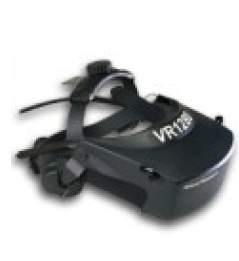
\includegraphics[width=\textwidth]{hmd.png}
                \caption{HMD}
                \label{fig:hmd}
        \end{subfigure}
        ~ %add desired spacing between images, e. g. ~, \quad, \qquad etc.
          %(or a blank line to force the subfigure onto a new line)
        \begin{subfigure}[b]{0.3\textwidth}
                \centering
                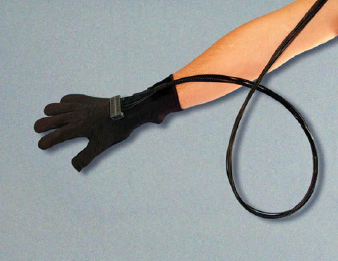
\includegraphics[width=\textwidth]{glove.png}
                \caption{5DT Ultra}
                \label{fig:ultra}
        \end{subfigure}
        \caption{Dispositivos de entrada}\label{fig:inputdev}
\end{figure}

\section{Context Aware Serious Games Framework for Sport and Health}

O \emph{SocialAware}~\cite{Hardy11} � um arcabou�o para a constru��o de servi�os cientes de contexto. No trabalho, � apresentado um conjunto de jogos s�rios para suporte a esporte e sa�de que, atrav�s do uso do arcabou�o, s�o transformados em jogos cientes de contexto. A captura do contexto do usu�rio, provendo servi�os de \textit{exergames} apropriados � vista como um aux�lio para solucionar muitos problemas de sa�de. Apesar de a maioria dos problemas de sa�de ocorrerem principalmente devido � falta de atividade f�sica, muitas s�o as pessoas que t�m motiva��o para praticar tais atividades. Os jogos s�rios para suporte a esportes e sa�de motivam as pessoas a praticarem exerc�cios durante a atividade do jogo, ou as ensinam sobre problemas de sa�de.

Na Figura~\ref{fig:hardy1}, ilustra-se a arquitetura do sistema e na Figura~\ref{fig:hardy2}, ilustra-se a interface de visualiza��o do \emph{SocialAware} mostrando servi�os diferentes em dois contextos distintos. Foram usados dados de acelera��o, temperatura e altura para calcular um n�vel de estresse e, dependendo do valor calculado, s�o sugeridos jogos diferentes. A captura de tela no topo mostra a interface durante o contexto \emph{no trabalho}. Prop�e-se que o usu�rio jogue um jogo ap�s ler um email importante, por exemplo. A tela de baixo mostra uma situa��o em casa. Os autores mencionam que n�o desejam que seus jogos sejam vistos como substitutos de esportes reais. Dessa forma, usando dados da previs�o do tempo e hora, pode-se sugerir atividades ao ar livre, se poss�vel. Se o sistema identificar que o usu�rio n�o realizou atividade aer�bica no dia anterior, por exemplo, pode sugerir uma caminhada ou um \emph{exergame} aer�bico.

\begin{figure}
        \centering
        \begin{subfigure}[b]{0.6\textwidth}
                \centering
                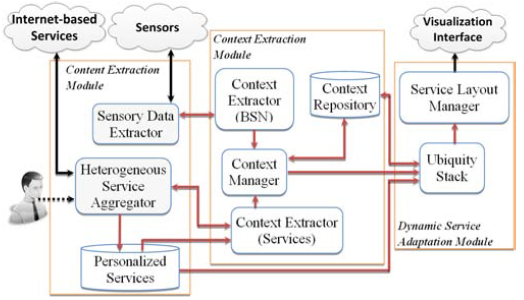
\includegraphics[width=\textwidth]{hardy1.png}
                \caption{Arquitetura do sistema}
                \label{fig:hardy1}
        \end{subfigure}%
        ~ %add desired spacing between images, e. g. ~, \quad, \qquad etc.
          %(or a blank line to force the subfigure onto a new line)
        \begin{subfigure}[b]{0.3\textwidth}
                \centering
                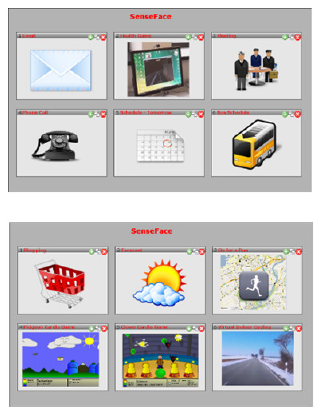
\includegraphics[width=\textwidth]{hardy2.png}
                \caption{Interface de visualiza��o em dois diferentes contextos}
                \label{fig:hardy2}
        \end{subfigure}
        \caption{\emph{SocialAware}}\label{fig:hardy}
\end{figure}

Estudos multidisciplinares recentes no dom�nio de sensores sem-fio, smartphones, redes sociais e comunica��o m�vel contribu�ram para a computa��o ciente de contexto. Dessa forma, � poss�vel capturar diferentes informa��es de contexto relacionadas a sinais vitais, como batimento card�aco, press�o sangu�nea, n�vel de glicose, condi��es do suor, etc. Al�m disso, podem ser capturadas a��es, como andar, dormir, dirigir, cair, correr, falar e conversar com um amigo, e tamb�m vari�veis de ambiente, como temperatura, umidade do ar, localiza��o, altitude, etc.

Extrair informa��es de contexto a partir de dados de sensores e informa��o multim�dia contida em servi�os heterog�neos traz dois desafios. Primeiramente, � necess�ria a extra��o em tempo real de conte�do multim�dia e de redes de sensores corporais para an�lise de contexto. Depois, � preciso aplicar a l�gica apropriada para extrair a informa��o de contexto das redes sociais e dados de sensores, agreg�-la e ent�o armazen�-la em um reposit�rio para ser usada em uma sele��o din�mica de jogos s�rios e servi�os de sa�de relevantes.

Tr�s m�dulos l�gicos s�o descritos para melhor representar o conceito:
\begin{enumerate}
  \item \textit{M�dulo de Extra��o de Conte�do}: respons�vel por extrair as informa��es de servi�os heterog�neos de Internet e da rede de sensores corporais.
  \item \textit{M�dulo de Extra��o de Contexto}: encontra o valor contextual de um servi�o. Extratores de conte�do recebem conte�do em tempo real de sensores e servi�os de Internet e passam o conte�do e os metadados de cada servi�o para os componentes apropriados.
  \item \textit{M�dulo de Adapta��o Din�mica de Servi�o}: mapeia dinamicamente um subconjunto de jogos s�rios e/ou servi�os relacionados � sa�de extra�dos de uma base de dados de Servi�os Personalizados, selecionando servi�os, jogos e n�veis de exerc�cio �nicos para cada pessoa.
\end{enumerate}

Para avaliar a efetividade do sistema proposto, foi conduzido um teste de avalia��o subjetiva entre maio e novembro de 2010, baseado em uma amostra de 95 pessoas, das quais 25\% s�o mulheres. A maior parte dos usu�rios tinham mais de 25 anos e 45 deles tinham menos de 25 anos. Todos os participantes utilizaram diversos servi�os de Internet em diferentes escalas nos �ltimos 4 a 6 anos. A ideia de utilizar sugest�es de servi�os din�micas foi fortemente aceita por 65\% dos usu�rios. Al�m disso, alguns usu�rios levantaram a quest�o da privacidade, enquanto outros usu�rios preocuparam-se com o pre�o dos sensores. Alguns demonstraram pessimismo devido � necessidade de sempre carregar os sensores para obter os servi�os.

\section{Serious Game Based on First Aid Education for Individuals with Autism Spectrum Disorder (ASD) Using Android Mobile Sevices}

Em \cite{Urturi11} � apresentado um conjunto de jogos para ajudar pessoas com Desordem do Espectro Autista (DEA). O paciente � motivado a jogar durante o seu progresso e atividades executadas durante o jogo s�o guardadas para gerar relat�rios, que ser�o acompanhados pelo paciente, sua fam�lia e/ou m�dicos. Primeiramente, um conjunto de mini-jogos � apresentado ao usu�rio, cada um com diferentes n�veis de dificuldade. Ap�s terminar a atividade, a aplica��o conecta-se com o servidor, acessa a base de dados e armazena os dados gerados durante o jogo, atualizando os registros daquele usu�rio, se necess�rio. Com os dados salvos, � gerado um relat�rio detalhado sobre o usu�rio, explicando em qual atividade foram cometidos erros e qual a poss�vel raz�o.

\vspace{5 mm}
\section{Game based Learning to Enhance Capabilities of Elderly People}

Arntzen~\cite{arntzen2011} discute os conceitos, realidade s�cio-econ�mica e requisitos t�cnicos para desenvolver jogos para idosos. Sabe-se que tecnologias de Realidade Virtual (RV) t�m o potencial de contribuir na melhoria de sess�es de terapia f�sica, tratamento do mal de Alzheimer, reabilita��o de infarto e assim por diante. O prop�sito do trabalho � desenvolver um jogo que contribua para melhorar as habilidades cognitivas e f�sicas de idosos ou deficientes. Desde o lan�amento do Nintendo Wii em 2008, os sensores de movimento nos jogos possibilitaram o conceito de \emph{exergames}. Al�m disso, novos jogos surgiram, provando a sua capacidade de melhorar as habilidades cognitivas atrav�s do est�mulo das atividades mentais.

Estudos recentes indicam que as pessoas podem evitar o decl�nio de habilidades cognitivas ou f�sicas se forem motivadas a exercitar seu c�rebro e corpo. Os novos sistemas de jogos t�m sido vistos com potencial por fisioterapeutas e outros profissionais de sa�de. Entretanto, desenvolver novos jogos requer entender as habilidades cognitivas e f�sicas dos idosos que geralmente diminuem com o tempo e, tamb�m, � necess�rio uma preocupa��o em rela��o � limita��o f�sica dos jogadores de idade avan�ada ou deficientes.

Ainda em~\cite{arntzen2011}, no projeto de jogo \emph{SmartBrain} aplicado � doen�a de Alzheimer, s�o utilizados meios para avaliar a escuta, reconhecimento de cores, avalia��o da mem�ria e execu��o de movimentos. O usu�rio n�o deve correr riscos de machucar-se devido a movimentos bruscos durante o jogo. � crucial que o jogador sinta-se seguro ao jogar.

\section{Conclus�o}

Nesta se��o foram apresentados os principais trabalhos que utilizam jogos com algum prop�sito relacionado � sa�de. As solu��es propostas s�o geralmente invasivas e, apesar terem como inten��o serem utilizadas pelos usu�rios por um longo per�odo, n�o existe a preocupa��o em manter o enredo do jogo atrativo para o usu�rio e criar nele a motiva��o para continuar jogando. A diferen�a para o trabalho aqui desenvolvido � o direcionamento para pessoas saud�veis e a preocupa��o em manter o projeto de jogo atrativo, embutindo nele os m�todos de monitoramento.
\chapter{Arcabou�o para a Aquisi��o de Dados de Sa�de Utilizando Jogos Eletr�nicos} \label{cap:arquitetura}

Este cap�tulo apresenta o arcabou�o que permite o desenvolvimento de jogos eletr�nicos para a aquisi��o de dados de sa�de. S�o apresentados os requisitos funcionais do arcabou�o e, em seguida, � feita uma descri��o detalhada da arquitetura do arcabou�o, mostrando seus componentes e funcionalidades. A arquitetura de coleta de dados est� embutida em um arcabou�o de desenvolvimento de Jogos Eletr�nicos que realiza a captura de sinais motores armaazenando esses dados e os enviando para um servidor atrav�s de um \textit{webservice}. O servidor possui mecanismos de multi-usu�rios, identifica��o dos clientes, rotinas de recebimento tornando poss�vel o acompanhamento dos dados motores para diferentes usu�rios. A proposta de arquitetura Cliente e Servidor do \textit{GAHME} apresentada nesse cap�tulo � fruto de uma colabora��o numa disserta��o de mestrado da UFCG ~\cite{antonio2013}.


\section{Requisitos do Arcabou�o}

Para possibilitar o desenvolvimento de jogos para captura de dados de sa�de, um arcabou�o deve permitir a aquisi��o e persist�ncia dos dados obtidos a partir da intera��o do usu�rio com sensores. A grande quantidade de dados coletada deve ser gerenciada pelo arcabou�o de monitoramento de sa�de, apoio � decis�o e processamento de informa��o cl�nica para auxiliar m�dicos em suas decis�es e melhorar o entendimento da din�mica da evolu��o de doen�as. O conhecimento m�dico � frequentemente atualizado e reavaliado para incluir a identifica��o de novos fatores de risco e novas evid�ncias de estudos cl�nicos. Os desafios enfrentados atualmente s�o: incorporar em sistemas pessoais de monitoramento de sa�de o conhecimento mais recente e baseado em evid�ncias; e transformar os dados coletados em conhecimento para suportar o processo de tomada de decis�o. A tecnologia pode ter um papel fundamental ao focar em uma abordagem baseada em conhecimento, como identifica��o de fatores de risco, testes diagn�sticos e novas evid�ncias de estudos cl�nicos, para integrar informa��es passadas e atuais de cada indiv�duo, junto com evid�ncias estat�sticas~\cite{Tartarisco20121296}.

Um requisito do arcabou�o � permitir que a coleta dos dados seja realizada de forma impercept�vel para o indiv�duo, embutida no enredo do pr�prio jogo no qual � utilizado. Outras informa��es relevantes, como idade, g�nero e medidas antropom�tricas, como peso e altura, podem ser obtidas em posteriormente, com o conhecimento do usu�rio, quando se fizer uso dos dados de sa�de coletados pelo arcabou�o.

\section{Arquitetura}

Na Figura~\ref{img:arquitetura}, apresenta-se uma vis�o geral da arquitetura da solu��o, que � constitu�da por quatro componentes: \emph{Web Service}, \emph{Gerenciador de Dados}, \emph{Analisador de Dados} e o \emph{Banco de Dados}. A estrutura est�tica do arcabou�o pode ser vista no diagrama de classes, na Figura~\ref{img:classd}. Na Figura~\ref{img:arquitetura_an}, apresenta-se a transfer�ncia de dados entre as classes do arcabou�o.

O processo se inicia com a aquisi��o dos dados dos sensores (1), que podem ser enviados para o \emph{webservice} e processados pela classe \texttt{ReadingResource} ou enviados por arquivos e processados pela classe \texttt{FileManager}, acessada atrav�s do \texttt{DataManager}. O \texttt{ReadingResource} envia os dados recebidos para o \texttt{DatabaseManager} (2), tamb�m acessado atrav�s do \texttt{DataManager}, para armazen�-los no \emph{banco de dados}. A partir da�, os dados podem ou n�o ser filtrados atrav�s do \texttt{FilterModule} pelas classes de filtro que implementam a interface \texttt{IFilter}, e depois enviados para o \texttt{DataAnalyzer} (3). No \texttt{DataAnalyzer}, os dados est�o prontos para serem processados pelas classes de an�lise que implementam a interface \texttt{IAnalyzer}. O \texttt{RuleManager} utiliza o \texttt{FileManager} para ler as regras de um arquivo (4) e as transfere para o \texttt{DataAnalyzer} (5), assim, os dados podem ser interpretados. O \texttt{DataAnalyzer} pode tamb�m enviar os dados para o \texttt{WriterModule} (6), que os escrever� em arquivo para visualiza��o em outros programas, ou utiliza��o em m�todos de aprendizado de m�quina, por exemplo.

\begin{figure}[!htb]
     \centering
     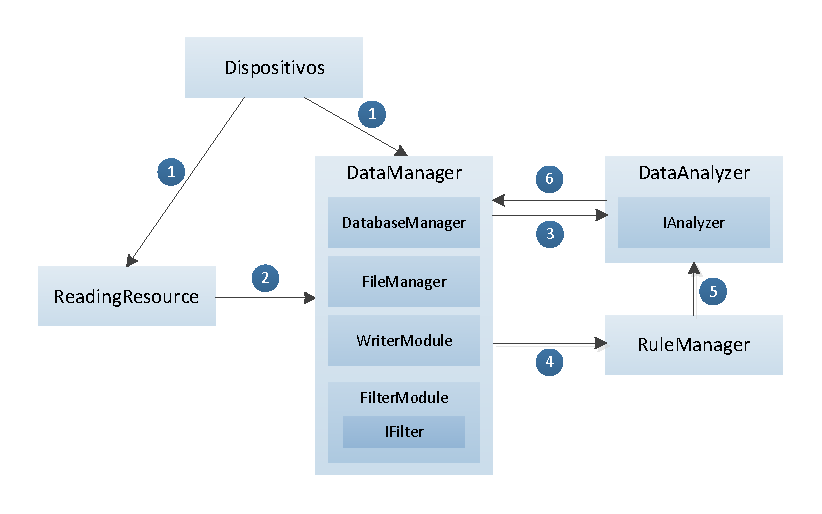
\includegraphics[width=1\textwidth]{arquitetura_alto_nivel.pdf}
     \caption{Transfer�ncia de Dados Dentro do Arcabou�o}
     \label{img:arquitetura_an}
\end{figure}

O envio dos dados dos usu�rios coletados com os dispositivos � feito atrav�s de uma requisi��o POST para o \textit{web service}. Os dados devem ser coletados durante uma sess�o completa do jogo, que dura de alguns segundos a alguns minutos, para depois serem estruturados e enviados para o \textit{web service}. O formato aceito pelas opera��es � o JSON (JavaScript Object Notation). Na Tabela~\ref{tab:operations}, ilustram-se as opera��es disponibilizadas pelo \textit{web service} e um exemplo de como os dados devem ser estruturados para cada opera��o.

\begin{figure}[!htb]
     \centering
     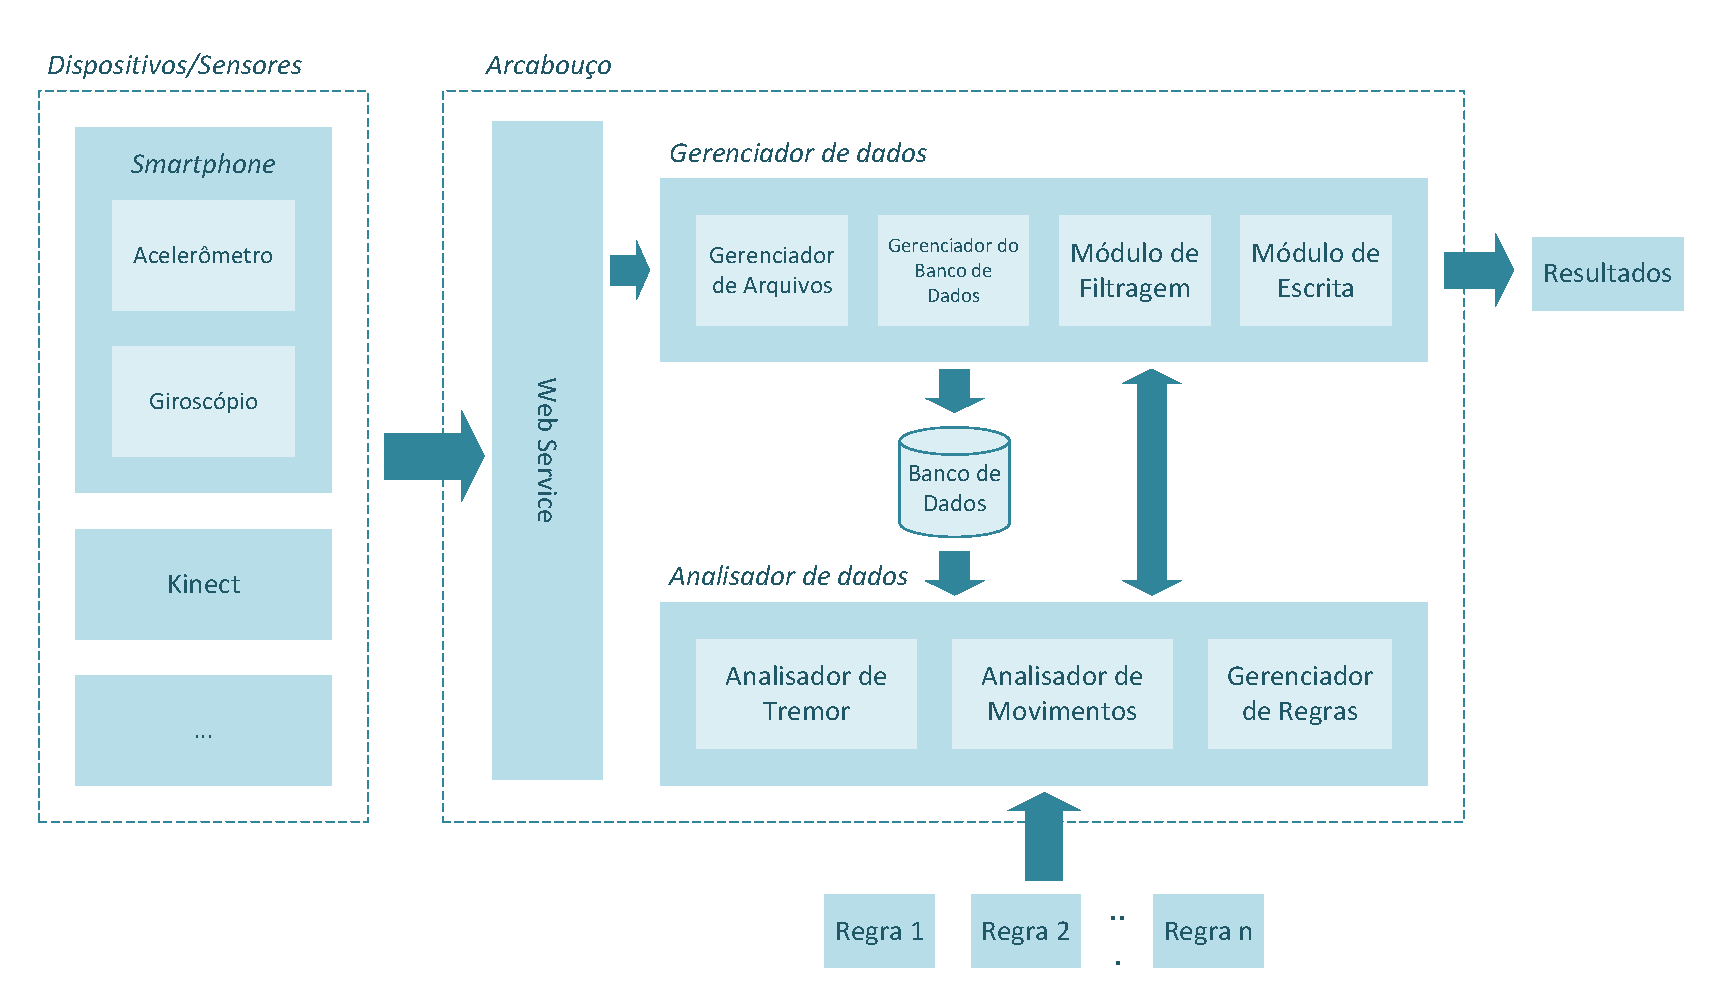
\includegraphics[width=1\textwidth]{arquitetura.pdf}
     \caption{Arquitetura do Arcabou�o}
     \label{img:arquitetura}
\end{figure}

\begin{figure}[!htb]
     \centering
     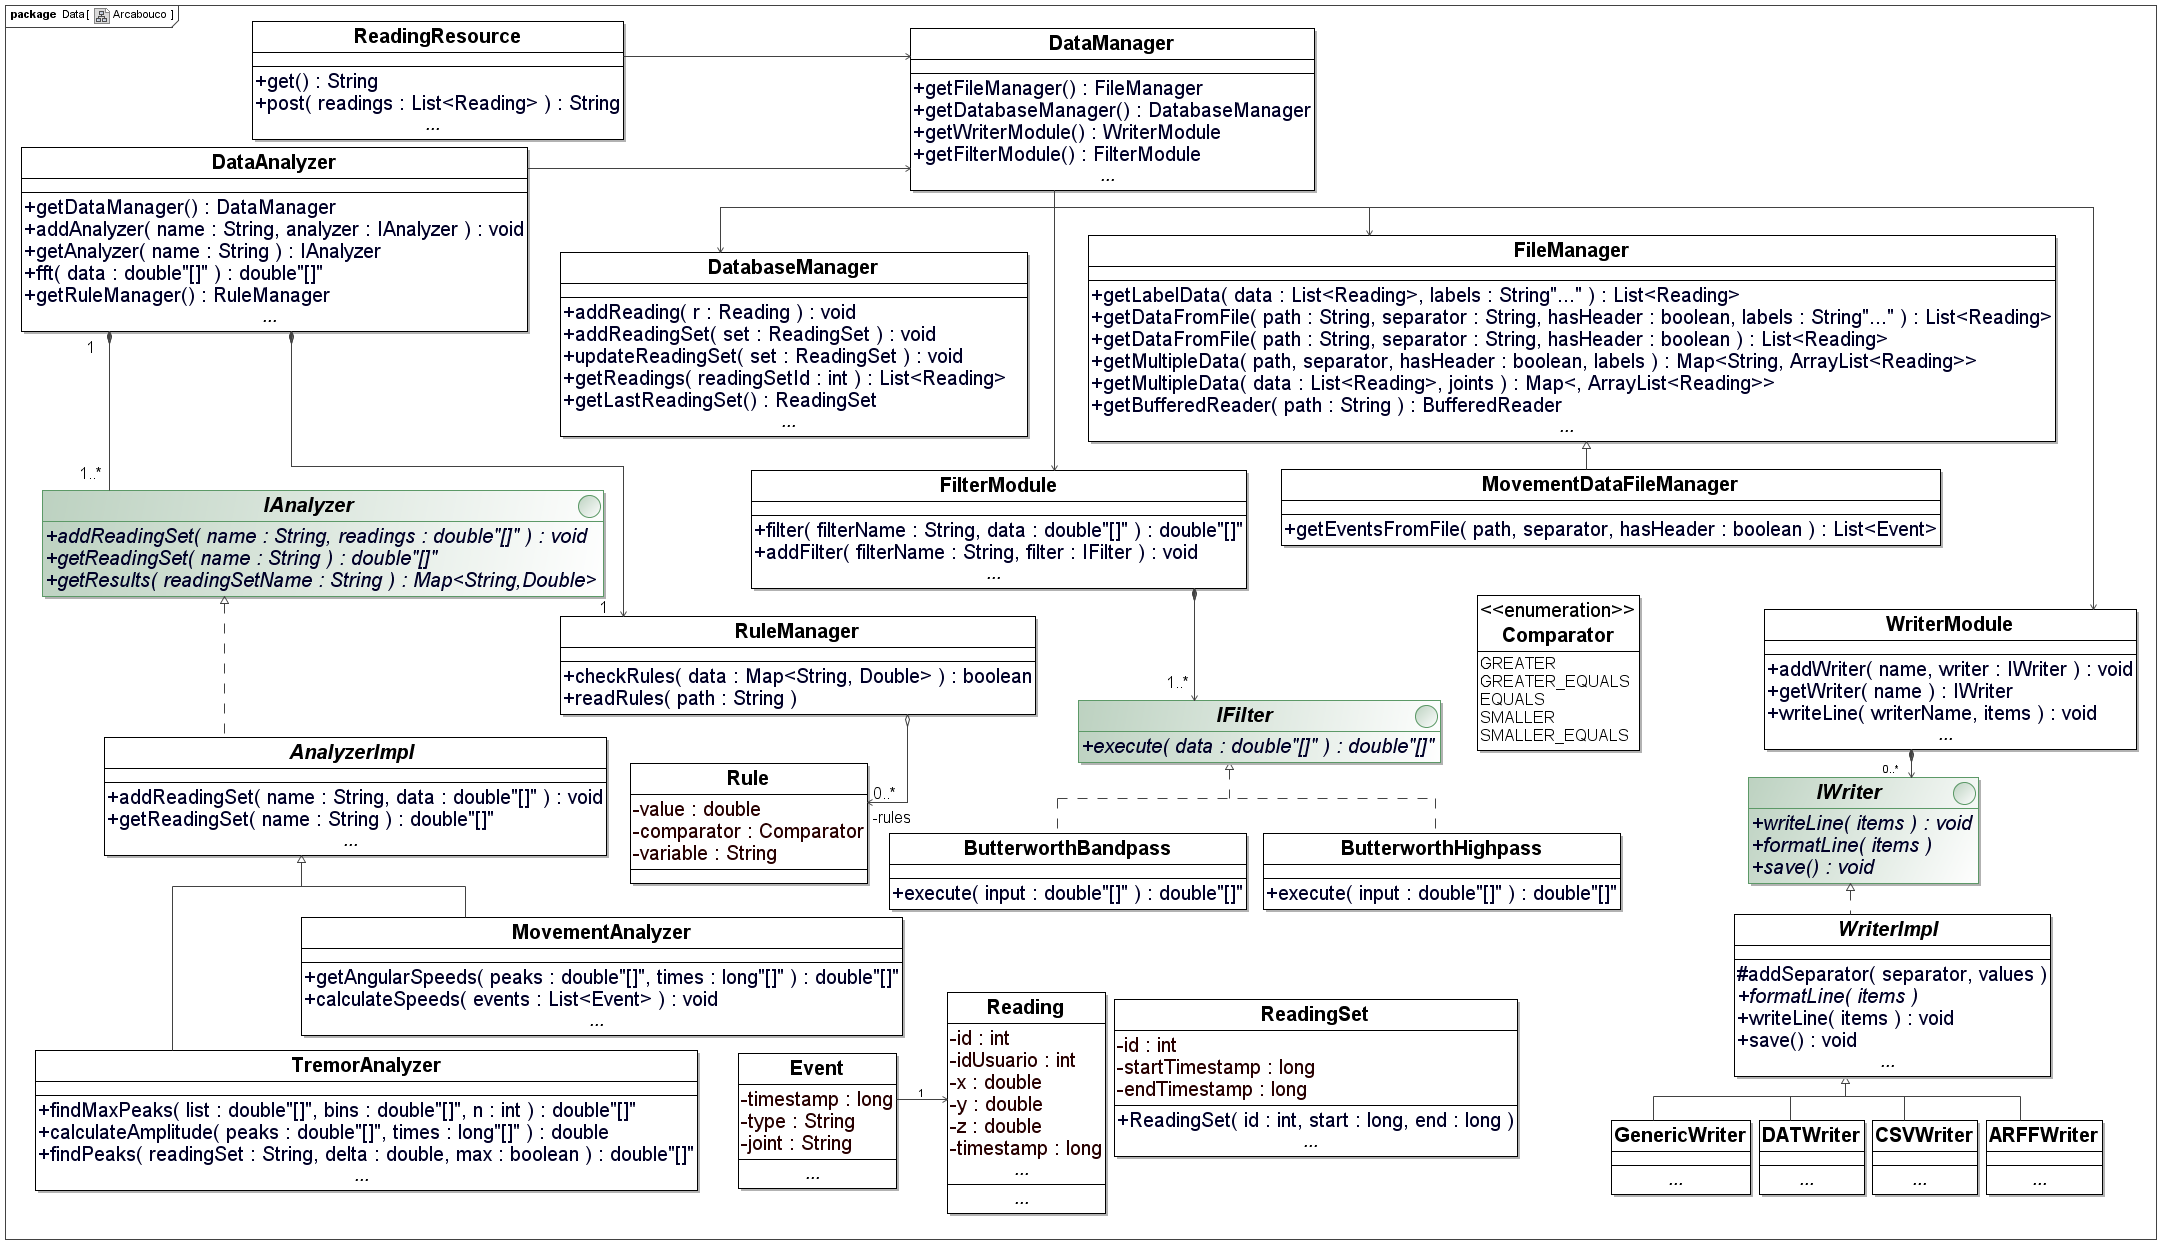
\includegraphics[width=1\textwidth]{class_diagram.png}
     \caption{Diagrama de Classes do Arcabou�o}
     \label{img:classd}
\end{figure}

\begin{table} 
\centering 
\caption{Opera��es disponibilizadas pelo \textit{web service}}
\begin{center}
    \begin{tabular}{ | l | c | l | }
        \hline
        Opera��o & M�todo & Exemplo \\ \hline
        cadastrarUsuario & POST & 
		\begin{minipage}{7cm}\begin{verbatim}
		
		{"id":2,"nome":"Ana",
		"masculino":false,
		"nascimento":"2012-11-28"}
		
		\end{verbatim}\end{minipage} \\ \hline
        obterToken & GET & - \\ \hline
        enviarDados & POST & 
		\begin{minipage}{7.5cm}\begin{verbatim}

		{"leitura":[{"id":0, 
		"idUsuario":1, "x":2.9097333, 
		"y":6.770132, "z":2.0355952, 
		"timestamp":1336134935706}, 
		{"id":0, "idUsuario":1, 
		"x":4.5565815, "y":4.9461093, 
		"z":1.4911331, 
		"timestamp":1336134935706}]}
		
		\end{verbatim}\end{minipage} \\ \hline
    \end{tabular}
\end{center}
\label{tab:operations}
\end{table}

\subsection{M�dulo Gerenciador de Dados} \label{sec:ger_dados}

O \emph{Gerenciador de Dados} possui subm�dulos respons�veis por fazer leitura, separa��o e filtragem dos dados, al�m do gerenciamento destes no Banco de Dados e escrita dos resultados disponibilizados pelo \emph{Analisador de Dados}. A classe \texttt{DataManager} implementa as funcionalidades do \emph{Gerenciador de Dados}, referenciando os quatro m�dulos, \emph{Gerenciador de Arquivos}, \emph{M�dulo de Escrita}, \emph{M�dulo de Filtragem} e \emph{Gerenciador do Banco de Dados}, que s�o explicados nas subse��es a seguir. A classe \texttt{DataManager} possui um construtor \texttt{DataManager(DatabaseManager, FileManager, WriterModule, FilterModule)}, que recebe como par�metros os quatro m�dulos. Dessa forma, � poss�vel aumentar a funcionalidade de cada um dos m�dulos estendendo suas respectivas classes por heran�a e adicionando a elas novos m�todos. A classe \texttt{MovementDataFileManager}, tratada mais adiante, � um exemplo de extens�o do \texttt{FileManager}.

O \emph{webservice}, implementado utilizando a biblioteca Jersey\footnote{Dispon�vel em: http://jersey.java.net/}, que facilita o desenvolvimento de \textit{RESTful webservices}. As requisi��es s�o enviadas para serem processadas pela classe \texttt{ReadingResource}, que � um \textit{web resource}, uma entidade que recebe requisi��es HTTP e envia respostas. Esta classe possui dois m�todos, o \texttt{get()} trata requisi��es \emph{GET}, retornando o identificador do �ltimo conjunto de leituras para controle do armazenamento no banco de dados; e o m�todo \texttt{post(List<Reading> readings)} processa os dados das leituras enviados atrav�s de requisi��es \emph{POST}, e convertidos de JSON para objetos Java pela biblioteca Jersey. A classe \texttt{ReadingResource} est� acoplada � classe \texttt{DataManager} e, atrav�s dela, tem acesso ao \emph{Gerenciador do Banco de Dados}. O \emph{webservice} pode ser instalado em qualquer \textit{web container}, como o Apache Tomcat\footnote{Dispon�vel em: http://tomcat.apache.org/} e o GlassFish\footnote{Dispon�vel em: http://glassfish.
java.net/}.

\subsubsection{Gerenciador de Arquivos}

A classe \texttt{FileManager} implementa o m�dulo \emph{Gerenciador de Arquivos}, e processa as opera��es de abertura de arquivos de dados delegadas pelo \emph{Gerenciador de Dados}. Esse m�dulo processa os dados recebidos, armazenando-os em dados estruturados para serem processado posteriormente pelo \emph{Analisador de Dados}. O dado estruturado aceito pelo \emph{Analisador de Dados} � composto por um r�tulo identificador do dado, uma marca de tempo com precis�o de milissegundos, e coordenadas x, y e z, cujo significado depende do tipo de sensor que as gera.

Os m�todos da classe \texttt{FileManager} s�o:
\begin{enumerate}
	\item \texttt{getLabelData(List<Reading> data, String... labels)} filtra os dados da lista de leituras \texttt{data}, retornando uma nova lista \texttt{List<Reading>} contendo apenas os dados com os r�tulos definidos em \texttt{labels}.
	\item \texttt{getDataFromFile(String path, String separator, boolean hasHeader)} l� os dados de um arquivo localizado no caminho \texttt{path}, cujos dados est�o separados pelo separador \texttt{separator} e definidos linha a linha. O par�metro \texttt{hasHeader} indica se o m�todo deve procurar por uma linha de cabe�alho na primeira linha do arquivo. Retorna uma \texttt{List<Reading>} com os dados.
	\item \label{getdatamethod} \texttt{getDataFromFile(String path, String separator, boolean hasHeader, String... labels)} estende a funcionalidade do m�todo anterior, retornando uma \texttt{List<Reading>} com os dados que possuem os r�tulos definidos em \texttt{labels}.
	\item \texttt{getMultipleData(String path, String separator, boolean hasHeader, String... labels)} possui a mesma fun��o que o m�todo~\ref{getdatamethod}, mas, diferente deste, retorna um \texttt{Map<String, List<Reading>>} onde cada chave do mapa � um r�tulo e indexa uma lista de eventos identificados pelo r�tulo.
	\item \texttt{getBufferedReader(String path)} retorna um \texttt{BufferedReader} para manipular o arquivo cujo caminho � especificado dem \texttt{path}.
\end{enumerate}

A classe \texttt{MovementDataFileManager} estende as funcionalidades do \texttt{FileManager}, adicionando um m�todo para leitura de eventos oriundos de jogos. Os eventos marcam o in�cio ou fim de um momento espec�fico do jogo no qual o jogador estar� executando um movimento que ser� enviado para an�lise.

\subsubsection{M�dulo de Escrita}

O \emph{M�dulo de Escrita} � implementado pela classe \texttt{WriterModule}, e � respons�vel pela sa�da dos dados processados pelo \emph{Analisador de Dados}. Os dados podem ser estruturados para serem mostrados em um programa de plotagem de gr�ficos, como o GNUPlot\footnote{Dispon�vel em: http://www.gnuplot.info/}, ou para servirem como entrada para mecanismos de aprendizado de m�quina. Os dados s�o escritos em CSV (\textit{Comma-separated Values}) ou em qualquer outro formato definido pelo usu�rio do arcabou�o. O m�dulo de escrita tamb�m suporta a escrita de arquivos ARFF, para serem processados pelo Weka\footnote{Dispon�vel em: http://www.cs.waikato.ac.nz/ml/weka/}. O \emph{M�dulo de Escrita} � extens�vel para permitir a gera��o de um formato de arquivo espec�fico. A cria��o de um novo arquivo de dados � feita atrav�s da extens�o da classe \texttt{WriterImpl} pela classe que se est� criando.

A interface \texttt{IWriter} define tr�s m�todos para manipular arquivos de dados:

\begin{enumerate}
	\item \label{formatlinemethod} \texttt{formatLine(Object... items)} formata os itens \texttt{items} adicionando separadores ou qualquer outra formata��o adicional definida na classe espec�fica de escrita que implementa \texttt{IWriter} ou estende \texttt{WriterImpl}.
	\item \texttt{writeLine(Object... items)} escreve uma nova linha no arquivo, seguindo a formata��o definida pelo m�todo~\ref{formatlinemethod}.
	\item \texttt{save()} fecha a \textit{stream} de escrita dedicada ao arquivo e salva o arquivo em disco.
\end{enumerate}

A classe \texttt{WriterImpl} implementa os m�todos comuns a todas as classes de escrita, definidos pela interface \texttt{IWriter}, fornecendo um m�todo adicional para incluir separadores entre os elementos de uma linha. Para definir um comportamento diferente daquele implementado por \texttt{WriterImpl}, deve-se implementar diretamente a interface \texttt{IWriter}.

\subsubsection{M�dulo de Filtragem}

O \emph{M�dulo de Filtragem} faz o pr�-processamento dos dados, selecionando apenas os espectros de frequ�ncia de interesse. A classe \texttt{FilterModule} implementa as funcionalidades do \emph{M�dulo de Filtragem}. Ela permite o gerenciamento de filtros, implementados em classes distintas, indexados por um nome e acessados por m�todos explicados a seguir.

\begin{enumerate}
	\item \texttt{addFilter(String filterName, IFilter filter)} adiciona um novo filtro \texttt{filter} indexado pelo nome \texttt{filterName}.
	\item \texttt{filter(String filterName, double[] data)} executa o filtro de nome \texttt{filterName} sobre os dados \texttt{data} e retorna um array \texttt{double[]} de mesmo tamanho que \texttt{data} com os dados filtrados.
\end{enumerate}

A interface \texttt{IFilter} define que as classes que implementarem filtros, dever�o receber os dados atrav�s do m�todo \texttt{execute(double[] data)}, e retorn�-los, depois de processados, dentro de um array \texttt{double[]}. Atualmente, duas classes de filtros est�o implementadas: \texttt{ButterworthHighpass}, um filtro passa-alta de frequ�ncia de corte de 1Hz e \texttt{ButterworthBandPass}, um filtro passa-faixa de frequ�ncias de corte de 2Hz e 8Hz, suficientes para identificar os tremores que ocorrem nas m�os.

Filtros passa-alta com frequ�ncia de corte de 1Hz s�o geralmente utilizados em aplica��es de an�lise de movimentos usando aceler�metros para remover mudan�as na orienta��o de segmentos do corpo, ajustes de postura e os efeitos da gravidade. Os componentes de frequ�ncia mais alta (2-16Hz) refletem as acelera��es de segmentos do corpo, tipicamente associadas com movimentos r�pidos, marcados por fases de acelera��o/desacelera��o~\cite{Bonato2004,Patel2009}.

\subsubsection{Gerenciador do Banco de Dados}

O \emph{Gerenciador do Banco de Dados}, implementado na classe \texttt{DatabaseManager} d� acesso ao mecanismo de persist�ncia do arcabou�o, que fornece opera��es de armazenamento e leitura dos dados coletados. A implementa��o do mecanismo de persist�ncia do arcabou�o baseia-se no Sistema de Gerenciamento de Banco de Dados (SGBD) Relacional MySQL\footnote{Dispon�vel em: http://dev.mysql.com/downloads/}. A comunica��o entre o \emph{Gerenciador de Dados} e o banco de dados MySQL � feita atrav�s do Hibernate\footnote{Dispon�vel em: http://www.hibernate.org/downloads}, um \textit{framework} para mapeamento objeto-relacional escrito na linguagem Java, permitindo consultas em SQL (\textit{Structured Query Language}) ou HQL (\textit{Hibernate Query Language}).

A classe \texttt{DatabaseManager} disponibiliza os seguintes m�todos para manipula��o dos dados:

\begin{enumerate}
	\item \texttt{getLastReadingSet()} Retorna o identificador \textit{id} do �ltimo \texttt{ReadingSet} gravado no banco de dados incrementado de 1. As novas leituras s�o adicionadas ao \texttt{ReadingSet} de identificador \textit{id} + 1. Isso permite adicionar um grande n�mero de leituras por etapas. Enquanto \texttt{getLastReadingSet()} n�o for chamado novamente, todas as leituras ser�o adicionadas ao \texttt{ReadingSet} que for retornado pelo m�todo.
	\item \texttt{addReading(Reading r)} adiciona uma nova leitura \texttt{r}.
	\item \texttt{addReadingSet(ReadingSet set)} adiciona um novo conjunto de leituras \texttt{set}.
	\item \texttt{updateReadingSet(ReadingSet set)} atualiza o conjunto de leituras \texttt{set} passado como atributo com suas novas informa��es. O identificador do \texttt{set} deve estar inicializado, para que este seja localizado no banco de dados.
	\item \texttt{getReadings(int readingSetId)} retorna uma \texttt{List<Reading>} com as leituras pertencentes ao conjunto de leituras de identificador \texttt{readingSetId}.
\end{enumerate}

\subsection{Analisador de Dados}

O \emph{Analisador de Dados}, implementado pela classe \texttt{DataAnalyzer}, realiza o processamento dos dados e retorna as informa��es necess�rias para a an�lise. A classe \texttt{IAnalyzer} especifica os m�todos que uma classe de an�lise de dados deve possuir. Uma nova classe deve implementar a interface \texttt{IAnalyzer}. Dois tipos de an�lise s�o suportadas atualmente, a an�lise de tremor e an�lise de movimentos, realizadas respectivamente pelo \emph{Analisador de Tremor} e \emph{Analisador de Movimentos}. A an�lise � feita baseada em regras providas ao sistema, utilizadas para definir como classificar as informa��es.

Os m�todos que uma nova classe de an�lise deve possuir s�o os seguintes:

\begin{enumerate}
	\item \texttt{addReadingSet(String name, double[] readings)} adiciona o novo conjunto de leituras \texttt{readings} sob o nome \texttt{name}.
	\item \texttt{getReadingSet(String name)} retorna o conjunto de leituras sob o nome \texttt{name}.
	\item \texttt{getResults(String readingSetName)} realiza a an�lise sobre o conjunto de leituras de nome \texttt{readingSetName} e retorna os resultados em um mapa \texttt{Map<String, Double>} onde a \textit{chave} � o nome de uma vari�vel de retorno da an�lise, e o \textit{valor} � o valor da vari�vel. A classe de an�lise deve apresentar todos os seus resultados dentro deste mapa, para avalia��o pelo \emph{Gerenciador de Regras}.
\end{enumerate}

Os m�todos disponibilizados pela classe \texttt{DataAnalyzer} s�o:

\begin{enumerate}
	\item \texttt{getDataManager()} retorna a inst�ncia do \emph{Gerenciador de Dados}.
	\item \texttt{getRuleManager()} retorna a inst�ncia do \emph{Gerenciador de Regras}.
	\item \texttt{addAnalyzer(String name, IAnalyzer analyzer)} adiciona uma nova classe de an�lise ao \emph{Analisador de Dados}, sob o nome \texttt{name} especificado.
	\item \texttt{getAnalyzer(String name)} retorna o analisador de nome \texttt{name}.
	\item \texttt{fft(double[] data)} executa a Transformada R�pida de Fourier (FFT) sobre os dados passados no array \texttt{data}. Retorna o resultado em um \textit{array} \texttt{double[]}.
\end{enumerate}

\subsubsection{Analisador de Tremor}

A implementa��o deste m�dulo � feita pela classe \texttt{TremorAnalyzer}, que processa o sinal do aceler�metro, realizando a an�lise de espectro para identificar as frequ�ncias de tremor predominantes. Pequenos aceler�metros s�o usados em muitas aplica��es cl�nicas, sendo bastante populares em aplica��es para medi��o de tremor, e s�o capazes de medir acelera��es menores que $0,02g$ ($1g = 9,807 m/s^2$, a acelera��o est�tica da gravidade)~\cite{Elble2005}. O sinal proveniente do aceler�metro de tr�s eixos � composto por coordenadas $(x, y, z)$, que representam a quantifica��o da for�a da gravidade sobre o eixo em um determinado momento. Na Figura~\ref{img:eixos}, ilustra-se um esquema de um aceler�metro e seus eixos $x, y$ e $z$, considerando o eixo $z$ perpendicular � for�a da gravidade $g$.

Para realizar a an�lise espectral do sinal do aceler�metro, � utilizada a Transformada R�pida de Fourier (\textit{FFT - Fast Fourier Transform}), acessada atrav�s do m�todo \texttt{fft(double[] data)}, dispon�vel na classe \texttt{DataAnalyzer}. A FFT transforma um sinal no dom�nio do tempo para o dom�nio de frequ�ncia. A maioria das an�lises espectrais � baseada na FFT, e sua simplicidade computacional permite uma implementa��o eficiente e an�lise de dados r�pida. A an�lise espectral � um popular m�todo para quantificar tremores, dada a caracter�stica oscilat�ria destes. A ideia � calcular a fun��o de densidade espectral de energia (\textit{Power Spectral Density - PSD}) em frequ�ncias diferentes por todo o espectro. A frequ�ncia dominante do tremor � evidente no maior pico na densidade espectral de energia~\cite{Riviere199777}.

\begin{figure}[!htb]
     \centering
     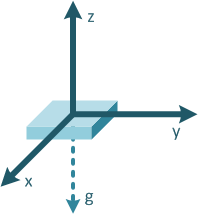
\includegraphics[width=.3\textwidth]{eixos.png}
     \caption{Eixos do aceler�metro}
     \label{img:eixos}
\end{figure}

Al�m dos m�todos especificados pela interface \texttt{IAnalyzer}, os seguintes m�todos s�o implementados na classe \texttt{TremorAnalyzer}:

\begin{enumerate}
	\item \texttt{findPeaks(String readingSet, double delta, boolean max)} encontra os picos m�nimos ou m�ximos no sinal contido no conjunto de leituras de nome \texttt{readingSet}. O par�metro \texttt{delta} � a diferen�a m�xima entre um pico local e geral, usado para encontrar os picos gerais. O valor de \texttt{delta} afeta o n�mero de picos encontrados. O par�metro \texttt{max} define se o m�todo deve retornar os picos m�ximos (se \texttt{max} for \texttt{true}) ou m�ximos e m�nimos (se \texttt{max} for \texttt{false}).
	\item \texttt{calculateAmplitude(double[] peaks, double[] times)} retorna a amplitude em cent�metros de um sinal de aceler�metro. A precis�o do m�todo depende da precis�o do aceler�metro.
\end{enumerate}

\subsubsection{Analisador de Movimentos}

O m�dulo \emph{Analisador de Movimentos} processa os dados obtidos do sensor de movimentos Kinect e medidas angulares obtidas de aceler�metros e girosc�pios para calcular a velocidade angular e �ngulo de inclina��o de segmentos do corpo. O Kinect � um sensor de movimento que funciona baseado em uma c�mera e um sensor de profundidade, captando coordenadas 3D de pontos com precis�o. Sua efic�cia na an�lise do movimento do corpo humano � comprovada, podendo substituir ferramentas de an�lise tridimensional quando uma alta acur�cia n�o � necess�ria~\cite{Tong2012,Pedro2012}. Aplica��es v�o desde a avalia��o do controle postural~\cite{Clark2012372}, � an�lise de marcha~\cite{gabelfull}.

Esse m�dulo � capaz de calcular a velocidade linear de movimento de pontos do corpo a partir dos dados do Kinect. Esses dados consistem de coordenadas espaciais $(x, y, z)$, que s�o as posi��es do esqueleto capturadas pelo Kinect, cujos valores s�o dados em unidades m�tricas. Na Figura~\ref{img:skeletonspace} � mostrado o \textit{Skeleton Space}, um sistema de coordenadas orientado para a direita, que posiciona o Kinect na origem, com o eixo z se estendendo na dire��o para qual o Kinect aponta. O eixo y positivo se estende para cima e o eixo x positivo se estende para direita.\footnote{Dispon�vel em: http://msdn.microsoft.com/pt-br/library/hh973078.aspx} A Figura~\ref{img:kinect} mostra a representa��o gr�fica das coordenadas da m�o esquerda ao acenar, obtidas do Kinect durante aproximadamente 10 segundos.

\begin{figure}[!htb]
     \centering
     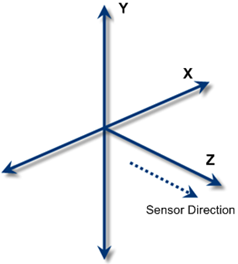
\includegraphics[width=.3\textwidth]{IC534689.png}
     \caption{O \textit{Skeleton Space}}
     \label{img:skeletonspace}
\end{figure}

\begin{figure}[!htb]
     \centering
     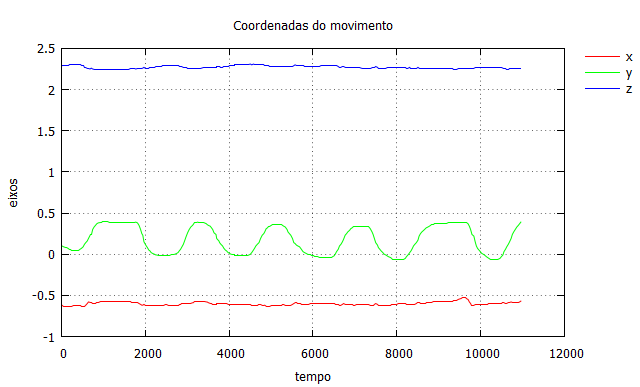
\includegraphics[width=.8\textwidth]{movimento_kinect.png}
     \caption{Plotagem das coordenadas da m�o esquerda}
     \label{img:kinect}
\end{figure}

\subsubsection{Gerenciador de Regras}

O \emph{Gerenciador de Regras} � implementado pela classe \texttt{RuleManager}, e permite especificar regras para classificar os dados provenientes do \emph{Analisador de Dados}. As regras permitem especificar condicionais que definir�o uma interpreta��o para os dados. As regras s�o especificadas atrav�s de arquivos, uma regra por linha, no formato \texttt{vari�vel sinal valor}, onde \texttt{vari�vel} � uma palavra, sem espa�os; \texttt{sinal} � um dos operadores \{\texttt{<}, \texttt{<=}, \texttt{==}, \texttt{>=}, \texttt{>}\} e \texttt{valor} � um decimal ou inteiro. No C�digo~\ref{rulesfile} � mostrado um exemplo de como estruturar o arquivo de regras.

\begin{lstlisting}[caption={Um exemplo de formato do arquivo de regras},label=rulesfile,numbers=none]
amplitude > 0
amplitude < 5
frequency >= 1
frequency < 9
\end{lstlisting}

As regras permitem verificar os resultados providos pelas classes analisadoras. Atrav�s das regras, por exemplo, podem ser providos intervalos normais de valores, e os valores obtidos do intera��o do usu�rio com os sensores s�o verificados para checar se s�o normais ou anormais. No caso de resultados anormais, � necess�ria uma investiga��o mais profunda para sua causa.

Os seguintes m�todos fazem parte da classe \texttt{RuleManager}:

\begin{enumerate}
	\item \texttt{readRules(String path)} carrega as regras contidas no arquivo provido em \texttt{path}. Este m�todo deve ser chamado antes do m�todo~\ref{checkrulesmethod}, ou a verifica��o das regras n�o ser� efetuada.
	\item \label{checkrulesmethod}\texttt{checkRules(Map<String, Double> data)} verifica se os dados providos em \texttt{data} obedecem �s regras definidas. O mapa \texttt{data} � provido por uma das classes de an�lise de dados.
\end{enumerate}

\section{Utilizando e Estendendo o Arcabou�o}

Nesta se��o, encontram-se os passos a serem seguidos para utilizar o arcabou�o e tamb�m estend�-lo. Por utilizar requisi��es HTTP e JSON para envio e representa��o dos dados, respectivamente, os m�todos para coleta de dados durante o jogo s�o independentes de linguagem. Entretanto, o arcabou�o foi feito em Java, e � necess�rio utilizar esta linguagem para usar as fun��es e partes do arcabou�o.

\subsection{Lendo e Armazenando os Dados de um Sensor Durante um Jogo}

A coleta dos dados deve ocorrer em uma frequ�ncia apropriada para captar atualiza��es significativas nos valores obtidos dos sensores. Para dados obtidos atrav�s de aceler�metros, por exemplo, � recomend�vel escolher a frequ�ncia de amostragem maior que a frequ�ncia de ocorr�ncia do evento que se deseja monitorar. Para identificar tremores, a frequ�ncia de amostragem deve ser pelo menos de 14 Hz para captar todos tipos de tremores que ocorrem nos membros (ver Tabela~\ref{tab:tremors}). Outros dados, como pulsa��o, podem ser lidos a uma taxa de amostragem menor, por n�o possuirem uma alta taxa de atualiza��o.

Para taxas de amostragem altas, recomenda-se que o envio para o \emph{webservice} seja feito de 1000 em 1000 leituras, aproximadamente, ou que todas as leituras sejam armazenadas em arquivo, para serem processadas posteriormente pelo arcabou�o. Para taxas de amostragem baixas, as leituras podem ser enviadas ao fim de uma sess�o de alguns minutos de jogo. O C�digo~\ref{coletaenvio} mostra um exemplo em Java de como as leituras devem ser armazenadas e enviadas.

O m�todo \texttt{enviar()} pode deter a execu��o do c�digo por algum tempo, devido � opera��o de enviar os dados pela rede. Para que nenhuma leitura do sensor seja perdida, no caso de uma taxa de amostragem alta, o ideal � que as opera��es dentro de \texttt{enviar()} sejam executadas em uma \textit{thread} diferente.

O objeto JSON \texttt{leitura}, mostrado no C�digo~\ref{objectjson} que representa uma leitura do sensor deve conter os atributos \textit{id}, \textit{idUsuario}, \textit{x}, \textit{y}, \textit{z} e \textit{timestamp}.

\begin{itemize}
	\item \textit{id} � o identificador da tabela do banco de dados, e pode ser enviado com valor 0, pois o objeto receber� o verdadeiro identificador quando for processado pelo \textit{Gerenciados de Dados}.
	\item \textit{idUsuario} � o identificador do usu�rio dentro da tabela de usu�rios no banco de dados, criada para uso futuro. O atributo \textit{timestamp} � a data e hora da leitura, convertida para um \texttt{long} que representa o n�mero de milissegundos desde 1 de Janeiro de 1970 at� a data e hora de leitura.
	\item \textit{x}, \textit{y} e \textit{z} s�o os valores decimais de uma leitura do sensor. Para aceler�metros, representam a acelera��o nos eixos x, y e z, respectivamente. Para o Kinect, a posi��o da pessoa no \textit{Skeleton Space}. Para outros sensores cuja leitura possui um n�mero de atributos menor que 3, apenas os atributos que possuem valor devem ser preenchidos e os atributos restantes ter�o valor 0. Para sensores cuja leitura retorna mais de 3 atributos, deve-se armazen�-los em arquivo e utilizar os m�todos apropriados do arcabou�o.
\end{itemize}

\begin{lstlisting}[caption={O objeto JSON \textit{leitura}},label=objectjson,numbers=none]
{"id":0,
"idUsuario":1,
"x":2.9097333,
"y":6.770132,
"z":2.0355952,
"timestamp":1336134935706}
\end{lstlisting}

\begin{lstlisting}[caption={Coleta e envio das leituras},label=coletaenvio,numbers=none]
int contador = 0;
final int MAX = 1000;
List<Leitura> dados = new ArrayList<Leitura>();

private void adicionaDado(Leitura dado){
    List<Leitura> copia;
    if (contador < MAX) {
        dados.add(dado);
        contador++;
    } else {
        copia = dados;
        dados.clear();
        enviar(copia);
    }
}
\end{lstlisting}

O envio de dados atrav�s de arquivos � mais flex�vel, pois � poss�vel estender o \texttt{FileManager} para permitir a leitura de um formato de dados espec�fico gravado em arquivo e sua posterior convers�o em uma estrutura de dados a ser utilizada no arcabou�o. Mais detalhes sobre a extens�o do \texttt{FileManager} s�o apresentados na Se��o~\ref{sec:extendingfile}.

\subsection{Estendendo o Arcabou�o} \label{sec:extending}

A estrutura do arcabou�o permite a extens�o de praticamente qualquer uma de suas partes. Esta se��o mostra os passos a serem seguidos para estender as partes do arcabou�o. As partes s�o extens�veis a partir do uso de interfaces, que reduz o acoplamento do c�digo.

\subsection{\textit{Classes de An�lise de Dados}}

Cada classe de an�lise de dados estende a interface \texttt{IAnalyzer}, que agrega os m�todos que definem o comportamento comum de todos os m�dulos analisadores de dados. Uma nova classe de an�lise deve implementar a interface \texttt{IAnalyzer} e prover a implementa��o concreta de seus m�todos, definindo seu c�digo espec�fico de an�lise.

A classe abstrata \texttt{AnalyzerImpl} possui a implementa��o dos m�todos \texttt{addReadingSet(String name, double[] data)} e \texttt{getReadingSet(String name)}, que � comum a todas as classes de an�lise. A nova classe de an�lise pode estender diretamente a classe \texttt{AnalyzerImpl} e implementar somente o m�todo \texttt{getResults(String name)}, ou, se necessitar  implementar um comportamento diferente para os dois m�todos \texttt{addReadingSet} e \texttt{getReadingSet}, a classe deve implementar diretamente a interface \texttt{IAnalyzer}. O C�digo~\ref{classeanalise} mostra um exemplo de implementa��o de uma nova classe de an�lise de dados.

\begin{lstlisting}[caption={Um Exemplo de Classe de An�lise de Dados},label=classeanalise,numbers=none]
public class GaitAnalyzer implements IAnalyzer {
   private Map<String, double[]> readings = 
      new HashMap<String, double[]>();
   private DataAnalyzer dataAnalyzer;

   public AnalyzerImpl(DataAnalyzer dataAnalyzer) {
      this.dataAnalyzer = dataAnalyzer;
   }

   @Override
   public void addReadingSet(String name, double[] data) {
      readings.put(name, data);
   }

   @Override
   public double[] getReadingSet(String name) {
      return readings.get(name);
   }

   @Override
   public Map<String, Double> getResults(String readingSetName) {
      // Definir c�digo espec�fico de an�lise de dados
   }
}
\end{lstlisting}

\subsection{\textit{Filtros}}

Novos filtros de dados podem ser adicionados, implementando a interface \texttt{IFilter}. As novas classes de filtros devem implementar a sua forma de filtragem dentro do m�todo \texttt{execute(double[] data)}, recebendo os dados atrav�s do par�metro \texttt{data} do m�todo. O C�digo~\ref{classefiltro} � um exemplo da estrutura de uma classe de filtragem de dados.

\begin{lstlisting}[caption={Um Exemplo de Classe de Filtragem de Dados},label=classefiltro,numbers=none]
public class SimpleLowPassFilter implements IFilter {
   @Override
   public double[] execute(double[] data) {
      // Realizar a filtragem
   }
}
\end{lstlisting}

\subsection{\textit{Gerenciador de Arquivos}} \label{sec:extendingfile}

A transfer�ncia de dados para o arcabou�o atrav�s de arquivos permite uma maior liberdade para representa��o dos dados. A transfer�ncia de dados pelo \emph{webservice} cobre as necessidades para a maioria dos sensores, entretanto, para formatos de dados especiais, � necess�rio recorrer � transfer�ncia por arquivos. A extens�o do \emph{Gerenciador de Arquivos} permite adicionar novos m�todos para leitura de dados e ainda assim utilizar toda a estrutura do arcabou�o. A classe \texttt{DataManager} pode ser estendida, para criar um novo \emph{Gerenciador de Arquivos}. O C�digo~\ref{gerarquivosclasse} mostra um exemplo de como estender o \emph{Gerenciador de Arquivos} (linha 1) e como utilizar o novo gerenciador \texttt{GaitDataFileManager} (linha 12).

\begin{lstlisting}[caption={Um Exemplo de Extens�o do Gerenciador de Arquivos},label=gerarquivosclasse,numbers=left]
public class GaitDataFileManager extends FileManager {
   
   public List<Stride> getGaitData(String path) {
      // Realizar a filtragem
   }
}

public class UsingTheFramework {

   public static void main(String[] args) {
      DatabaseManager dbMan = new DatabaseManager();
      FileManager fileMan = new GaitDataFileManager();
      WriterModule writerMod = new WriterModule();
      FilterModule filterMod = new FilterModule();

      DataManager dataMan = new DataManager(dbMan, fileMan, writerMod, filterMod);
   }
}
\end{lstlisting}

\subsection{\textit{Classes de Escrita de Dados}}

A extens�o das classes de escrita de dados � feita atrav�s da implementa��o da interface \texttt{IWriter} ou extens�o da classe \texttt{WriterImpl}, sendo o primeiro caso indicado quando se quer os m�todos \texttt{writeLine}, \texttt{formatLine} e \texttt{save} com comportamentos diferentes dos m�todos implementados pela classe \texttt{WriterImpl}. Um exemplo de cria��o de uma nova classe de escrita de dados encontra-se no C�digo~\ref{classeescrita}.

\begin{lstlisting}[caption={Um Exemplo de Classe de Escrita de Dados},label=classeescrita,numbers=none]
public class DashSeparatedValuesWriter extends WriterImpl {

	public DashSeparatedValuesWriter(String path, String... titles) throws IOException {
		super(path, titles);
	}

	@Override
	public String formatLine(Object... items) {
		return addSeparator("-", items);
	}
}
\end{lstlisting}

\section{Conclus�o}

Neste cap�tulo, foi apresentada a estrutura geral do arcabou�o, detalhando suas partes e opera��es. Foram apresentadas as opera��es disponibilizadas pelo \emph{webservice} e as classes, e seus respectivos m�todos, que fazem parte do arcabou�o. Por fim, foram descritas a estrutura��o do c�digo na constru��o de um jogo e a forma de extens�o do arcabou�o, para adicionar novas funcionalidades.
\chapter{Estudo de Caso} \label{cap:estudo}

Este cap�tulo apresentada o desenvolvimento de dois estudos de caso para demonstrar o uso do arcabou�o para captura de dados de sa�de utilizando jogos eletr�nicos. Os dois jogos, desenvolvidos em coopera��o com o IFAL, utilizam as opera��es de captura de dados oferecidas pelo arcabou�o. O cap�tulo apresenta uma descri��o dos dois jogos, os tipos de dados que capturam e a forma como interagem com o arcabou�o.

\section{\emph{Pinball World}}

O \emph{Pinball World} � um mini-jogo casual em terceira pessoa onde o jogador dever� controlar uma bola de \textit{pinball} em busca de completar os objetivos do jogo. Os caminhos a serem percorridos durante o jogo apresentam obst�culos, como buracos, paredes e rampas, dos quais o jogador deve desviar a bola, coletando o m�ximo de estrelas de ouro que encontrar pelo caminho. O jogo se ambienta num cen�rio de ru�nas, ao redor de plantas e uma queda d'�gua, transmitindo uma sensa��o de tranquilidade ao jogador. Na Figura~\ref{img:pw1}, ilustram-se capturas de tela do \emph{Pinball World}.

\begin{figure}[!htb]
     \centering
     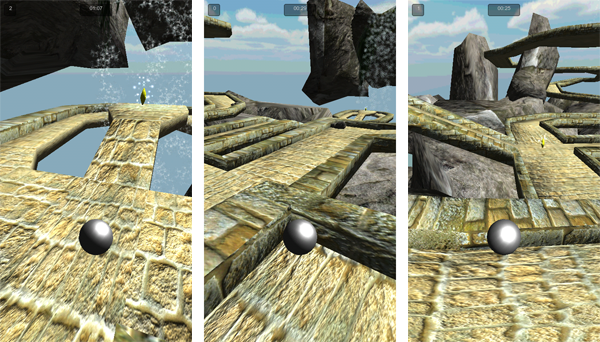
\includegraphics[scale=.6]{pinball_world.png}
     \caption{O Jogo \emph{Pinball World}}
     \label{img:pw1}
\end{figure}

O jogador dever� mover a bola de \textit{pinball} inclinando o dispositivo para esquerda, direita, frente e tr�s, controlando-a atrav�s dos caminhos e obst�culos, ou deixando-a descer livremente por rampas. A finalidade de controlar a bola apenas inclinando o dispositivo, atrav�s de seu aceler�metro, � capturar os n�veis de tremor de movimento e repouso do jogador. O tremor de movimento � capturado durante os momentos em que o jogador precisa movimentar o dispositivo para controlar a bola e desviar de obst�culos. Em outro momento, quando o jogador mant�m o dispositivo parado e precisa apenas visualizar o trajeto da bola, � poss�vel capturar o tremor de repouso.

\subsection{Desenvolvimento do Jogo}

O \emph{Pinball World} foi desenvolvido para a plataforma Android\footnote{Mais informa��es em: http://www.android.com} no \emph{Unity}\footnote{Dispon�vel em: http://www.unity3d.com}, uma IDE (\textit{Integrated Development Environment}) e motor de jogos 3D multi-plataforma desenvolvido pela \emph{Unity Technologies}, que permite o desenvolvimento de jogos para \textit{plugins} web, plataformas \textit{desktop}, videogames e dispositivos m�veis. A codifica��o em Unity � feita atrav�s de scripts, que podem ser em tr�s linguagens, JavaScript, C\# ou Boo. O uso de scripts dentro do Unity consiste de anexar objetos de script customizados chamados de \emph{comportamentos} aos objetos do jogo. Fun��es espec�ficas dentro dos objetos de script s�o chamadas quando ocorrem certos eventos.

As coordenadas do aceler�metro s�o capturadas a uma taxa de amostragem de 16Hz durante o curso do jogo, que requer conex�o com a Internet para que as coordenadas sejam enviadas para o \textit{webservice}. De acordo com a Tabela~\ref{tab:tremors}~\cite{albanese2012}, uma taxa de amostragem de 16Hz � suficiente para capturar os tipos de tremores que ocorrem nas m�os e membros. As a��es de capturar as coordenadas e envi�-las para o \textit{webservice} s�o impercept�veis para o jogador. No jogo as coordenadas s�o capturadas no m�todo \texttt{Update}, que � o m�todo que atualiza o desenho dos gr�ficos. O C�digo~\ref{updatemethod} mostra o m�todo \texttt{Update}. A vari�vel \texttt{taxaDeColeta} (linha 1) define o tempo em segundos entre cada leitura de dados (um total de 16 por segundo) e \texttt{quantidadeAColetar} (linha 3) define o n�mero de leituras a serem feitas, antes de enviar as leituras para o \emph{webservice}. O m�todo \texttt{coletarLeituras} (linha 16) realiza as leituras de dados, transformando-os em formato JSON, e o m�todo \texttt{enviarLeituras} (linha 19) envia os dados para o \emph{webservice}. O C�digo~\ref{enviarmedicoesmethod} mostra o m�todo \texttt{enviarLeituras}, que envia uma requisi��o POST para o \emph{webservice}, atrav�s de sua opera��o \texttt{enviarDados}.

\begin{lstlisting}[caption={O M�todo \texttt{Update}},label=updatemethod,numbers=left]
var taxaDeColeta:float = 0.0625;
var proximaColeta = 0.0;
var quantidadeAColetar:int = 120;

function Update () {
   acceleration = Input.acceleration;

   if(Input.GetKeyDown(KeyCode.Escape)){
      Application.Quit();
   }

   if(Time.time > proximaColeta){
      totalColetado++;
      proximaColeta = Time.time + taxaDeColeta;

      coletarLeituras();

      if(totalColetado >= quantidadeAColetar){
         enviarLeituras();
      }
   }
}
\end{lstlisting}

\begin{lstlisting}[caption={O M�todo \texttt{enviarLeituras}},label=enviarmedicoesmethod,numbers=none]
function enviarLeituras () {
   var jsonString:String = "{\"leitura\":["+medicoesStr+"]}";
   var postUrl = "http://"+Configuracoes.ip+":8080/accelerometer-webservice/enviarDados";
   var encoding = new System.Text.UTF8Encoding();
   var postHeader = new Hashtable();

   postHeader.Add("Content-Type", "application/json");
   postHeader.Add("Content-Length", jsonString.Length);

   var request = WWW(postUrl,encoding.GetBytes(jsonString), postHeader);

   limparLeituras();

   yield request;

   if (request.error != null) {
      Debug.Log("request error: " + request.error);
   } else {
      Debug.Log("request success");
   }
}
\end{lstlisting}

Na Figura~\ref{img:acc}, ilustram-se os dados do aceler�metro capturados durante uma sess�o do jogo \emph{Pinball World}. O sinal do eixo z foi filtrado usando um filtro passa alta com frequ�ncia de corte de 1 Hz.

\begin{table} 
\centering 
\caption{Tipos de tremor, diferenciados pela frequ�ncia, amplitude e in�cio em rela��o a movimentos volunt�rios}
\begin{center}
    \begin{tabular}{ | l | p{2.5cm} | p{2.5cm} | p{2.5cm} | p{3.5cm} | }
        \hline
        Frequ�ncia & Tipo de tremor & Amplitude & Lado predominante & Rela��o com movimento volunt�rio \\ \hline
        1-4 Hz & Cerebelar & M�dia-Alta & Membros & Postural, a��o \\ \hline
        3-5 Hz & Espec�fico de tarefa & Baixa-M�dia & M�o & Escrita, segurar talheres, tocar instrumentos \\ \hline
        4-5 Hz & Parkinsoniano & M�dia-Alta & Membros, mand�bula & Repouso \\ \hline
        5-8 Hz & Essencial & M�dia-Alta & Membros, cabe�a, voz & Postural \\ \hline
        8-12 Hz & Fisiol�gico & M�dia & Membros & Postural \\ \hline
        14-16 Hz & Ortost�tico & Baixa-M�dia & Pernas, tronco & Ficar de p� \\ \hline
    \end{tabular}
\end{center}
\label{tab:tremors}
\end{table}

\begin{figure}[!htb]
     \centering
     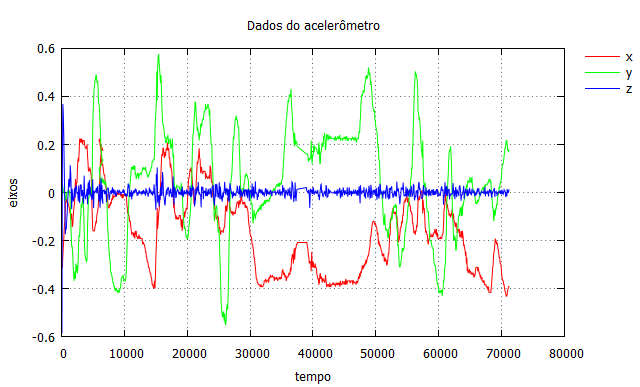
\includegraphics[width=.8\textwidth]{accelerometer_game.png}
     \caption{Plotagem das coordenadas da m�o esquerda}
     \label{img:acc}
\end{figure}

\section{\emph{Catch the Spheres}}

O \emph{Catch the Spheres} � um mini-jogo em terceira pessoa no qual o jogador, atrav�s de seu personagem, deve capturar ou desviar de bolas que v�m em sua dire��o. Existem dois tipos de bolas: azuis e vermelhas. Inicialmente, todas as bolas s�o vermelhas e algumas destas mudam para a cor azul ao se aproximarem do jogador. O tempo para a bola mudar de cor pode ser menor ou maior, a depender do n�vel de dificuldade selecionado. Um personagem no centro do cen�rio replica todos os movimentos executados pelo jogador e capturados atrav�s do Kinect. Deve-se tocar as bolas azuis com os p�s ou as m�os e desviar das bolas vermelhas. Na Figura~\ref{img:catch}, ilustra-se uma captura de tela do jogo \emph{Catch the Spheres}.

\begin{figure}[!htb]
     \centering
     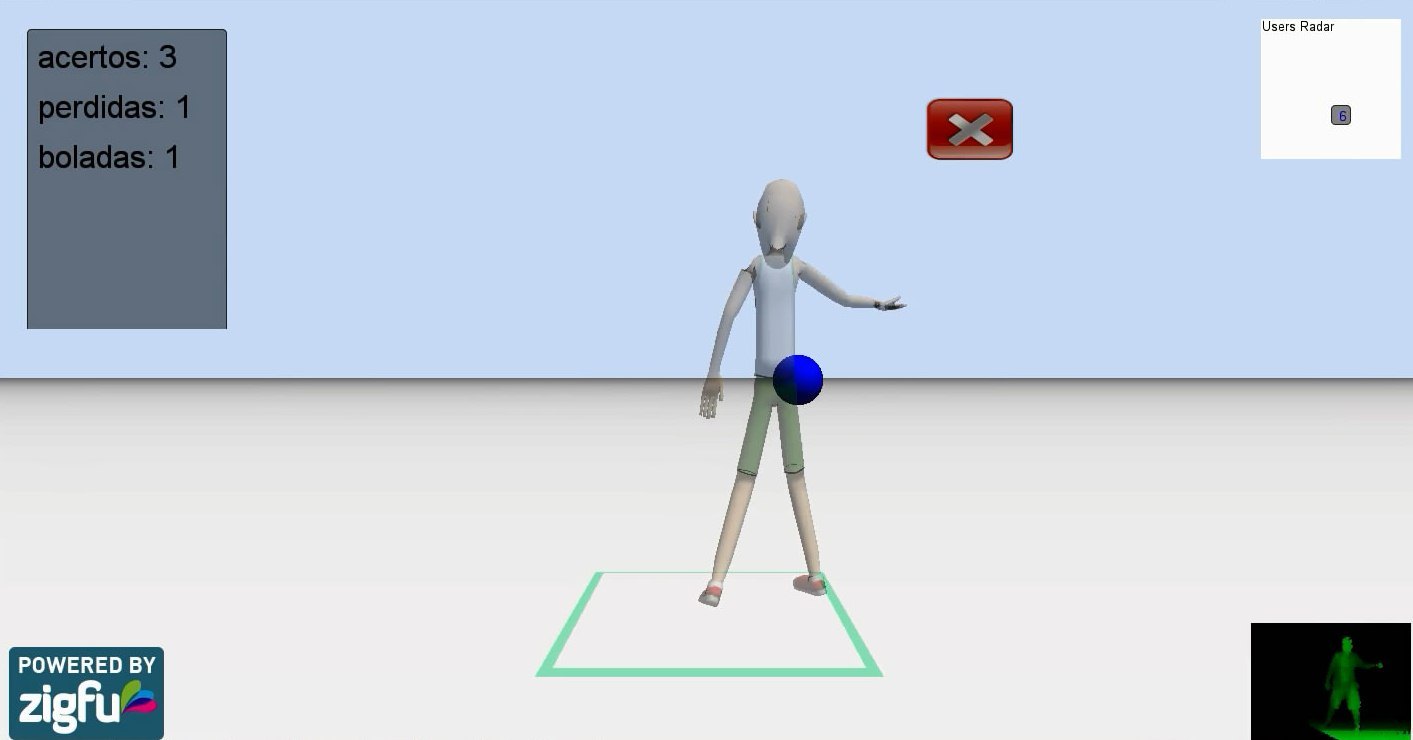
\includegraphics[width=.8\textwidth]{catch-the-spheres.jpg}
     \caption{O jogo \emph{Catch the Spheres}}
     \label{img:catch}
\end{figure}

A finalidade do jogo � capturar dados do movimento do jogador enquanto ele executa as a��es espec�ficas do jogo. O intervalo de tempo entre o momento em que a bola muda de cor e o momento em que a bola � capturada pelo jogador mede o reflexo do jogador, enquanto que a velocidade dos seus membros � calculada atrav�s da dist�ncia percorrida pelas m�os ou p�s para capturar as bolas.

\subsection{Desenvolvimento do Jogo}

O \emph{Catch the Spheres} foi desenvolvido para Windows, tamb�m no \textit{Unity}. Uma vez que n�o existe suporte nativo ao Kinect no \textit{Unity}, a integra��o entre o Kinect e o \textit{Unity} � feita atrav�s do plugin \textit{ZigFu}\footnote{Dispon�vel em: http://zigfu.com}.

Para \emph{Catch the Spheres}, a linguagem de script utilizada foi JavaScript. A base de captura de dados do jogo � a classe \texttt{ZigSkeletonHealth}, cuja classe base � a \texttt{ZigSkeleton}, que define o comportamento do personagem no jogo, repetindo os movimentos do jogador de acordo com as posi��es das partes do corpo obtidas do Kinect. A classe \texttt{ZigSkeletonHealth} coleta as posi��es do jogador em tempo real atrav�s do m�todo \texttt{UpdatePosition}, mostrado no C�digo~\ref{updatepositionmethod}. O m�todo \texttt{UpdatePosition} � chamado sempre que uma nova posi��o � recebida do Kinect. A classe \texttt{ZigSkeletonHealth} intercepta a atualiza��o das posi��es, primeiro gravando-as em um registro (linhas 2-6), depois enviando-as para \texttt{ZigSkeleton}, respons�vel por atualizar as posi��es do personagem dentro do jogo (linha 7).

\begin{lstlisting}[caption={O M�todo \texttt{UpdatePosition}},label=updatepositionmethod,numbers=left]
public override void UpdatePosition(ZigJointId joint, Vector3 position){
   if (logging) {
      healthGameLog.SendMessage("NewLineHealth", SendMessageOptions.DontRequireReceiver);
      healthGameLog.SendMessage("UpdateMessageHealth",joint.ToString(), SendMessageOptions.DontRequireReceiver);
      healthGameLog.SendMessage("UpdatePositionHealth",position, SendMessageOptions.DontRequireReceiver);
   }
   base.UpdatePosition(joint, position);
}
\end{lstlisting}

As coordenadas de posi��o 3D capturadas pelo Kinect s�o armazenadas em arquivo para serem enviadas posteriormente para o \textit{webservice}.
S�o coletadas as posi��es 3D da cabe�a, pesco�o, tronco, cintura, ombros, cotovelos, m�os, joelhos, quadris, tornozelo e p�s. Al�m das posi��es, o jogo mant�m registro dos eventos do jogo, tais como: o momento em que a bola muda de cor, o momento em que acerta o jogador, o momento em que � capturada e qual membro tocou a bola, e o momento em que a bola � perdida pelo jogador.

Os eventos do jogo s�o registrados pelo \textit{scriptEsfera.js}. Este script est� acoplado ao objeto da esfera e controla todos os comportamentos relacionados a ela. No C�digo~\ref{mudardecormethod}, � mostrado o m�todo respons�vel por mudar a cor da esfera e gravar o evento de mudan�a de cor no registro. Esse evento de mudan�a de cor, junto com os outros eventos relacionados � esfera, s�o capturados pelo \textit{scriptEsfera.js}.

\begin{lstlisting}[caption={O M�todo \texttt{mudarDeCor}},label=mudardecormethod,numbers=none]
function mudarDeCor(){
	renderer.material.color = Color.blue;
	healthGameLog.SendMessage("NewLineGame", SendMessageOptions.DontRequireReceiver);
	healthGameLog.SendMessage("NewMessageGame", "BALL-CHANGED-COLOR", SendMessageOptions.DontRequireReceiver);
	mudouDeCor = true;
}
\end{lstlisting}

O C�digo~\ref{eventos} mostra um trecho do registro de eventos que acontecem durante uma partida do jogo. \emph{BALL-THROW} indica a instancia��o de uma bola; \emph{BALL INITIAL POSITION} registra a posi��o inicial da bola; \emph{BALL-CHANGED-COLOR} registra o momento em que a bola muda de cor; \emph{BALL-LOST} registra que o jogador n�o capturou a bola; \emph{BALL-TOUCHED-POSITION} indica o momento em que a bola muda de cor e qual parte do corpo a tocou. No C�digo~\ref{posicoes}, � mostrado um trecho do registro de posi��es de cada parte do corpo durante uma partida do jogo. Cada linha mostra a data e hora, parte do corpo e as coordenadas x, y e z de sua posi��o. Essas informa��es s�o essenciais para que o \emph{M�dulo de An�lise de Movimento} possa calcular os dados baseado nos eventos e posi��es do jogador.

\begin{lstlisting}[caption={Registro de eventos do jogo},label=eventos,numbers=none]
25/01/2013 14:46:02.039;BALL-THROW;
25/01/2013 14:46:02.039;BALL INITIAL POSITION;(0.7, 0.8, 15.0);
25/01/2013 14:46:04.429;BALL-LOST;
25/01/2013 14:46:06.042;BALL-THROW;
25/01/2013 14:46:06.042;BALL INITIAL POSITION;(0.7, -0.1, 15.0);
25/01/2013 14:46:08.096;BALL-CHANGED-COLOR;
25/01/2013 14:46:09.892;BALL-TOUCHED-POSITION;(-1.1, -0.3, 0.1);LeftFoot;
\end{lstlisting}

\begin{lstlisting}[caption={Registro de posi��es do jogador durante jogo},label=posicoes,numbers=none]
25/01/2013 14:45:50.043;Head;-272.6079;882.585;-2700.646
25/01/2013 14:45:50.046;Neck;-271.4839;703.1649;-2718.727
25/01/2013 14:45:50.047;Torso;-240.7533;353.3502;-2744.491
25/01/2013 14:45:50.047;Waist;-234.5915;286.2368;-2706.167
25/01/2013 14:45:50.047;LeftShoulder;-465.3047;635.5613;-2740.658
25/01/2013 14:45:50.047;LeftElbow;-706.9146;748.0466;-2709.664
25/01/2013 14:45:50.048;LeftWrist;-974.8713;893.9808;-2650.611
25/01/2013 14:45:50.048;LeftHand;-1043.088;943.8502;-2600.744
25/01/2013 14:45:50.048;RightShoulder;-97.64243;602.8177;-2742.309
25/01/2013 14:45:50.049;RightElbow;27.13427;350.8448;-2744.681
25/01/2013 14:45:50.049;RightWrist;105.6349;94.18786;-2619.21
25/01/2013 14:45:50.049;RightHand;117.9995;8.172159;-2596.19
25/01/2013 14:45:50.050;LeftHip;-307.1635;199.0239;-2694.262
25/01/2013 14:45:50.050;LeftKnee;-302.8908;-343.2552;-2741.012
25/01/2013 14:45:50.050;LeftAnkle;-286.5235;-734.1376;-2757.292
25/01/2013 14:45:50.050;LeftFoot;-340.947;-798.0139;-2696.392
25/01/2013 14:45:50.051;RightHip;-149.0519;206.6668;-2707.094
25/01/2013 14:45:50.051;RightKnee;-13.03214;-357.2705;-2691.866
25/01/2013 14:45:50.051;RightAnkle;57.49874;-736.5664;-2653.726
25/01/2013 14:45:50.051;RightFoot;83.5181;-798.9075;-2605.077
\end{lstlisting}

\section{Avalia��o Experimental}

Dezoito pessoas com idades entre 17 e 27 anos (14 homens e 4 mulheres) do Laborat�rio Embedded da Universidade Federal de Campina Grande e do Instituto Federal de Alagoas foram selecionadas para jogar o \emph{Pinball World} e o \emph{Catch the Spheres}, para testar e responder um question�rio para avaliar o grau de divers�o dos jogos, sua facilidade de entendimento e possibilidade de inser��o de monitoramento atrav�s de jogos na rotina das pessoas. Buscou-se tamb�m validar o funcionamento do arcabou�o, avaliando a possibilidade de capturar corretamente os dados de sa�de. O seguinte procedimento foi utilizado para executar as sess�es de teste:

\begin{enumerate}
	\item O usu�rio joga o \emph{Catch the Spheres} por, aproximadamente, 1 minuto e 30 segundos em ritmo normal.
	\item Pede-se ao usu�rio para jogar novamente, simulando movimentos lentos, por mais 1 minuto e 30 segundos.
	\item O usu�rio joga o \emph{Pinball World} por, aproximadamente, 1 minuto e 30 segundos.
	\item Ao final, o usu�rio � informado do prop�sito dos jogos e responde o question�rio.
\end{enumerate}

Para identificar a possibilidade de integrar o monitoramento da sa�de do jogador atrav�s de jogos eletr�nicos � sua rotina di�ria, foi utilizada a abordagem \textit{Goal, Question, Metric} (GQM)~\cite{van1999goal}. GQM � uma abordagem hier�rquica que inicia com objetivo principal e o divide em atividades que podem ser mensuradas durante a execu��o do projeto. � uma abordagem para integrar objetivos a modelos de processos de software, produtos e perspectivas de qualidade de interesse, baseado nas necessidades do projeto e da organiza��o. Foi preparado o question�rio GQM mostrado na Tabela~\ref{tab:gqm} para avaliar a possibilidade de monitorar dados motores de forma n�o invasiva na rotina di�ria das pessoas.

\begin{center}
\begin{longtable}{|p{\textwidth}|}
\caption{O Question�rio GQM}\\
\hline
\endfirsthead
\multicolumn{1}{c}%
{\tablename\ \thetable\ -- \textit{Continua��o da p�gina anterior}} \\
\hline
\endhead
\hline \multicolumn{1}{r}{\textit{Continua na pr�xima p�gina}} \\
\endfoot
\hline
\endlastfoot
\textbf{\textit{Objetivo principal}}: Avaliar a possibilidade de monitorar dados motores de forma n�o invasiva na rotina di�ria das pessoas. \\ \hline
\textbf{\textit{Objetivo 1}}: Avaliar o n�vel de divers�o proporcionado pelo jogo do ponto de vista do jogador. \\ \hline
\textit{Quest�o 1.1}: O usu�rio considera o jogo divertido? \\ \hline
\textit{M�trica 1.1.1}: Nota em uma escala de 1 a 5 qual para quantificar o grau de divers�o do jogo. \\ \hline
\textit{M�trica 1.1.2}: O jogador sente-se imerso no jogo com a abordagem de captura dos movimentos? (Sim/ N�o) \\ \hline
\textit{Quest�o 1.2}: O jogador agregaria esse tipo de jogo em sua rotina di�ria? (Sim/ N�o) \\ \hline
\textit{M�trica 1.2.1}: Se o usu�rio tivesse adquirido esse jogo, com que frequencia o utilizaria durante a semana? (1 vez/3 vezes/Todos os dias/Nunca usaria) \\ \hline
\textit{Quest�o 1.3}: O jogo � casual? \\ \hline
\textit{M�trica 1.3.1}: O jogador considera o jogo simples, sem muitas regras, de f�cil entendimento e para diferentes idades? (Sim/ N�o) \\ \hline
\textit{M�trica 1.3.2}: O jogador se sentiria motivado a jogar esse jogo? (Sim/N�o) \\ \hline
\textit{Quest�o 1.4}: O usu�rio costuma jogar jogos desse estilo normalmente? \\ \hline
\textit{M�trica 1.4.1}: O jogador tem o costume de jogar esses jogos casuais em casa, durante uma viagem? (Sim/ N�o) \\ \hline
\textit{Quest�o 1.5}: O usu�rio acha que o monitoramento de sa�de atrav�s de um jogo � invasivo? \\ \hline
\textit{M�trica 1.4.1}: Sendo os dados acess�veis somente sob sob permiss�o, o usu�rio acha que o monitoramento de sa�de atrav�s de jogos � invasivo? (Sim/ N�o) \\ \hline
\textbf{\textit{Objetivo 2}}: Avaliar os requisitos n�o-funcionais do jogo do ponto de vista do jogador. \\ \hline
\textit{Quest�o 2.1}: Qual a opini�o do jogador sobre o jogo? \\ \hline
\textit{M�trica 2.1.1}: Nota de 1 a 5 para avaliar usabilidade. \\ \hline
\textit{Quest�o 2.2}: Qual a opini�o do jogador sobre a jogabilidade do jogo? \\ \hline
\textit{M�trica 2.2.1}: Nota de 1 a 5 para avaliar jogabilidade. \\ \hline
\textit{Quest�o 2.3}: Esse jogo seria adequado para uma crian�a/adulto/idoso? \\ \hline
\textit{M�trica 2.3.1}: Uma crian�a/adulto/idoso estaria segura jogando esse jogo, ao efetuar os movimentos dos bra�os e das pernas? (Sim/N�o) \\ \hline
\textit{M�trica 2.3.2}: Qual a sua opini�o do jogador sobre a faixa et�ria do jogo? (Livre/Crian�as/Adultos/Idosos)
\label{tab:gqm}
\end{longtable}
\end{center}

Tendo em vista o objetivo principal definido no question�rio GQM acima, o question�rio a seguir foi aplicado a 18 pessoas, na faixa de 19 a 27 anos, perguntando-as sobre sua opini�o em rela��o ao jogo. A preocupa��o principal foi avaliar o grau de entretenimento dos jogadores, a possibilidade de integrar jogos para monitoramento na rotina dos jogadores, motiva��o para jogar, seguran�a e opini�o do jogador em rela��o ao monitoramento da sa�de.

\begin{enumerate}
  \item Numa escala de 1 a 5 qual o grau de divers�o do jogo?
  \item Voc� agregaria um jogo desse estilo em sua rotina di�ria? (Sim/N�o)
  \item Se voc� tivesse adquirido esse jogo, com que frequ�ncia voc� o utilizaria durante a semana? (1 vez/3 vezes/Todo dia/Nunca)
  \item Voc� considera o jogo simples, sem muitas regras, de f�cil entedimento e para diferentes idade? (Sim/N�o)
  \item Voc� sentiria motivado a jogar esse jogo? (Sim/N�o)
  \item Voc� tem o costume de jogar esses jogos casuais? (Sim/N�o)
  \item Uma crian�a estaria segura jogando esse jogo, ao efetuar os movimentos dos bra�os e das pernas (Sim/N�o)
  \item Um adulto estaria seguro ao jogar esse jogo, ao efetuar os movimentos dos bra�os e das pernas (Sim/N�o)
  \item Um idoso estaria seguro ao jogar esse jogo, ao efetuar os movimentos dos bra�os e das pernas (Sim/N�o)
  \item A qual faixa et�ria voc� acha o jogo � direcionado? (Livre/Crian�as/Adultos/Idosos)
  \item Sendo os dados acess�veis somente sob sob permiss�o, voc� acha que o monitoramento de sa�de atrav�s de jogos � invasivo? (Sim/N�o)
\end{enumerate}

Os resultados do question�rio s�o apresentados na Figura~\ref{result}. O resultado foi positivo, considerando as respostas relativas � aceita��o dos jogos pelas pessoas. Com as respostas positivas obtidas foram atingidos os dois objetivos definidos no question�rio GQM:

\begin{description}
	\item[Objetivo 1] Avaliar o n�vel de divers�o proporcionado pelo jogo do ponto de vista do jogador.
	\item[Objetivo 2] Avaliar os requisitos n�o-funcionais do jogo do ponto de vista do jogador.
\end{description}

O Objetivo 1 pode ser considerado alcan�ado, devido �s respostas alcan�adas com as perguntas 1, 2, 3 e 5 do question�rio. Das 18 pessoas, 61\% (11 pessoas) acharam os jogos divertidos, atribuindo a eles uma nota 4 (de 1 a 5), 67\% (12 pessoas) agregariam jogos casuais � sua rotina di�ria, 61\% (11 pessoas) os jogariam 3 vezes por semana e 94\% (17 pessoas) sentir-se-iam motivadas a jogar os jogos. Atrav�s dessas respostas, � poss�vel concluir que jogos casuais no estilo dos apresentados nesse estudo poderiam proporcionar divers�o aos jogadores, enquanto realizam o monitoramento em sua rotina di�ria.

Quanto ao Objetivo 2, a resposta dos jogadores indica que os jogos possuem caracter�sticas como facilidade de entendimento e seguran�a, apesar de requererem que o usu�rio jogue movimentando-se. Todos os jogadores consideraram o jogo de f�cil entendimento e que � seguro para crian�as e adultos. Entretanto, 72\% (13 pessoas) acha que os jogos n�o seriam seguros para idosos. Um total de 80\% acha que monitorar a sa�de atrav�s de jogos n�o � um procedimento invasivo. A aceita��o dos usu�rios e opini�o quanto � facilidade de uso tornam poss�vel concluir que o monitoramento atrav�s de jogos poderia ser realizado sem maiores problemas, capturando corretamente os dados de sa�de dos jogadores.

Apesar de o question�rio ter avaliado a opini�o dos jogadores quanto aos dois jogos apresentados, � poss�vel generalizar e dizer que essas opini�es s�o v�lidas para outros jogos no mesmo estilo, desde que possuam um enredo atrativo. Um projeto de jogo melhor elaborado poderia ter obtido uma aceita��o ainda mais positiva.

\begin{figure}
        \centering
        \begin{subfigure}[b]{0.3\textwidth}
                \centering
                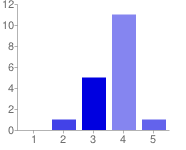
\includegraphics[width=\textwidth]{chart_1.png}
                \caption{Pergunta 1 (1: 0\%; 2: 6\%; 3: 28\%; 4: 61\%; 5: 6\%)}
                \label{fig:question1}
        \end{subfigure}%
        ~ %add desired spacing between images, e. g. ~, \quad, \qquad etc.
          %(or a blank line to force the subfigure onto a new line)
        \begin{subfigure}[b]{0.3\textwidth}
                \centering
                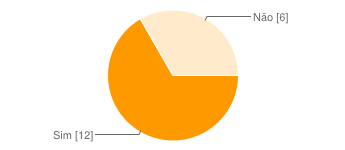
\includegraphics[width=\textwidth]{chart_2.png}
                \caption{Pergunta 2 (Sim: 67\%; N�o: 33\%)}
                \label{fig:question2}
        \end{subfigure}
        ~
        \begin{subfigure}[b]{0.3\textwidth}
                \centering
                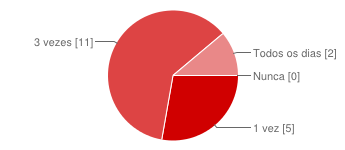
\includegraphics[width=\textwidth]{chart_3.png}
                \caption{Pergunta 3 (1 vez: 28\%; 3 vezes: 61\%; Todos os dias: 11\%; Nunca: 0\%)}
                \label{fig:question3}
        \end{subfigure}

        \begin{subfigure}[b]{0.3\textwidth}
                \centering
                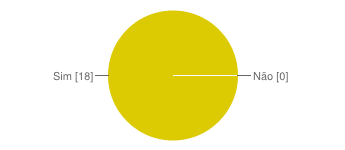
\includegraphics[width=\textwidth]{chart_4.png}
                \caption{Pergunta 4 (Sim: 100\%)}
                \label{fig:question4}
        \end{subfigure}
        ~
        \begin{subfigure}[b]{0.3\textwidth}
                \centering
                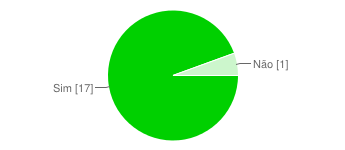
\includegraphics[width=\textwidth]{chart_5.png}
                \caption{Pergunta 5 (Sim: 94\%; N�o: 6\%)}
                \label{fig:question5}
        \end{subfigure}
        ~
        \begin{subfigure}[b]{0.3\textwidth}
                \centering
                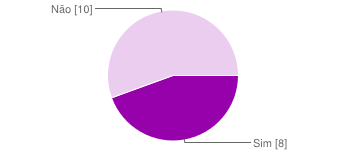
\includegraphics[width=\textwidth]{chart_6.png}
                \caption{Pergunta 6 (Sim: 44\%; N�o: 56\%)}
                \label{fig:question6}
        \end{subfigure}

        \begin{subfigure}[b]{0.3\textwidth}
                \centering
                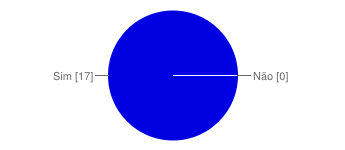
\includegraphics[width=\textwidth]{chart_7.png}
                \caption{Pergunta 7 (Sim: 100\%)}
                \label{fig:question7}
        \end{subfigure}
        ~
        \begin{subfigure}[b]{0.3\textwidth}
                \centering
                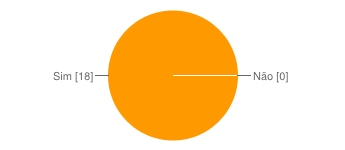
\includegraphics[width=\textwidth]{chart_8.png}
                \caption{Pergunta 8 (Sim: 100\%)}
                \label{fig:question8}
        \end{subfigure}
        ~
        \begin{subfigure}[b]{0.3\textwidth}
                \centering
                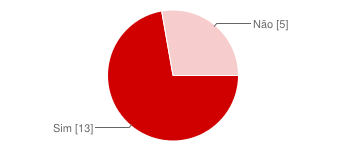
\includegraphics[width=\textwidth]{chart_9.png}
                \caption{Pergunta 9 (Sim: 72\%; N�o: 28\%)}
                \label{fig:question9}
        \end{subfigure}

        \begin{subfigure}[b]{0.3\textwidth}
                \centering
                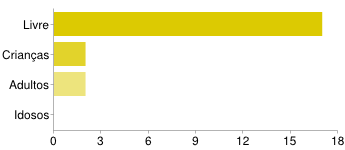
\includegraphics[width=\textwidth]{chart_10.png}
                \caption{Pergunta 10 (Livre: 80\%; Crian�as: 10\%; Adultos: 10\%; Idosos: 0\%)}
                \label{fig:question10}
        \end{subfigure}
        ~
        \begin{subfigure}[b]{0.3\textwidth}
                \centering
                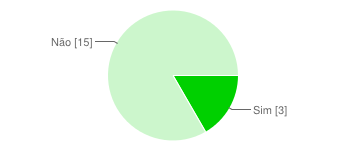
\includegraphics[width=\textwidth]{chart_11.png}
                \caption{Pergunta 11 (Sim: 17\%; N�o: 83\%)}
                \label{fig:question11}
        \end{subfigure}
        \caption{Respostas do question�rio}\label{result}
\end{figure}

Ao analisar o movimento normal e o movimento lento de todos os usu�rios durante o jogo \emph{Catch the Spheres}, foi poss�vel constatar a redu��o ou, no m�nimo, uma altera��o na velocidade de movimento. Ap�s remover as amostras de dados inv�lidas (por exemplo, aquelas em que o jogador j� estava com o membro na posi��o exata de capturar a bola), foi calculada a m�dia (VM) e desvio padr�o (DP) da velocidade dos membros dos jogadores, mostrados na Tabela~\ref{tab:vel}.

\begin{table} 
\centering 
\caption{Varia��o de Velocidade em Duas Sess�es do Jogo \emph{Catch the Spheres}}
\begin{center}
    \begin{tabular}{ | c | c | c | c | c | c | }
        \hline
        VM (Movimento r�pido) & DP & VM (Movimento lento) & DP & Varia��o M�dia & DP \\ \hline
        35,32cm/s & 6,34 & 21,83cm/s & 7,42 & 13,49cm/s & 1,6 \\ \hline	
    \end{tabular}
\end{center}
\label{tab:vel}
\end{table}

Tamb�m, com a an�lise dos dados coletados durante as sess�es do \emph{Pinball World}, foi poss�vel verificar que nenhum dos usu�rios possui amplitude de tremor significativa. A m�dia das frequ�ncias de tremor � de 2,85Hz, com magnitude m�dia de 3,15. Os desvios padr�o para a magnitude e frequ�ncia, respectivamente, s�o: 1,24 e 1,7, indicando que a m�dia da magnitude e frequ�ncia de tremor dos jogadores � bastante pr�xima.

\section{Conclus�o}

Este cap�tulo mostrou como exemplos de jogos simples podem explorar superficialmente o potencial do arcabou�o. Jogos mais complexos podem contemplar a��es para prover um suporte mais completo ao monitoramento da sa�de. Um projeto de jogo mais elaborado, aliado a uma melhor apresenta��o gr�fica, entre outros itens de projetos de jogos que mant�m a aten��o do jogador, podem criar uma experi�ncia de monitoramento cont�nua e prolongada.
\chapter{Considera��es Finais} \label{cap:conclusao}

%3) Detalhe melhor a conclus�o... est� muito resumida. Fale sobre o que foi apresentado, as contribui��es, limita��es e trabalhos futuros.

Ultimamente, t�m surgido diversos jogos com o prop�sito de motivar o jogador a exercitar-se ou realizar monitoramento. Entretanto, estas solu��es requerem que o jogador habitue-se com um estilo de jogo que, geralmente, n�o est� presente em seu cotidiano. Al�m disso, as a��es realizadas dentro do jogo s�o incomuns para o tipo de jogo geralmente preferido pelos jogadores.

A contribui��o desse trabalho � um arcabou�o que permite realizar a aquisi��o de dados de sa�de em jogos eletr�nicos. Sua forma de captura permite que ele receba os dados de monitoramento de qualquer jogo, se os dados estiverem no formato requerido pelo arcabou�o, em JSON, ou um formato espec�fico definido pelo desenvolvedor. � necess�rio apenas adaptar os movimentos necess�rios do jogador durante o jogo, de forma que os sensores de movimento capturem os dados corretamente para obten��o de informa��o de sa�de. A inclus�o da aquisi��o de dados de sa�de de forma invis�vel para o usu�rio permite realizar o monitoramento em jogos n�o direcionados para a sa�de, como os de a��o, aventura, \emph{arcade}, etc.

De acordo com as respostas obtidas dos jogadores durante os testes, os jogadores consideraram os jogos desenvolvidos divertidos e de f�cil entendimento. A maioria deles declarou sentir-se motivada a jogar o jogo, incluindo-o em sua rotina di�ria. Apesar dos experimentos n�o terem sido realizados com pessoas doentes, devido � dificuldade em se conseguir autoriza��o do Conselho de �tica, atrav�s dos experimentos realizados foi poss�vel verificar que, se ocorrerem movimentos incomuns, � poss�vel detect�-los atrav�s dos m�todos corretos.

Alguns sensores ainda n�o suportados pelo arcabou�o, como monitor de batimentos card�acos vest�vel e sensor de peso, j� s�o utilizados no contexto de jogos e isso abre margem para extens�o e evolu��o do arcabou�o, gerando novas solu��es de monitoramento no contexto de assist�ncia m�dica pervasiva. A partir do uso do arcabou�o, torna-se simples o suporte ao uso desses sensores na rotina do indiv�duo de forma n�o perturbadora, sem afetar a sua rotina di�ria.

Atrav�s de t�cnicas de aprendizado de m�quina, como redes neurais e m�quinas de vetores de suporte, � poss�vel classificar os dados e obter informa��es que n�o s�o descobertas somente com o uso de regras. A adi��o de um m�dulo de aprendizado de m�quina � uma extens�o valiosa do arcabou�o.

Outro trabalho futuro a ser realizado � adicionar um m�dulo estat�stico ao arcabou�o, que encontre medidas estat�sticas para os par�metros capturados, informando qual o intervalo de normalidade para determinados valores. O m�dulo estat�stico pode prover fun��es �teis, como verificar se os movimentos do usu�rio est�o dentro do normal, quando comparados a uma amostra, dentro de uma popula��o.

%%%%%%%%%%%%%%%%%%%%%%%%%%%%%%%%%%%%%%%%%%%%%%%%%%%%%%%%%%%%%%%%%%%%%%%%%%%%%%%%
%% Bibliografia
%% Coloque suas referencias no arquivo ref.bib e descomente as proximas duas linhas

\bibliographystyle{plain}
\bibliography{ref}

%%%%%%%%%%%%%%%%%%%%%%%%%%%%%%%%%%%%%%%%%%%%%%%%%%%%%%%%%%%%%%%%%%%%%%%%%%%%%%%%
%% Apendice
% Caso seja necessario algum apendice, descomente a proxima linha.

%\appendix
%\chapter{Question�rio}
%\chapter{Principais Algoritmos do Arcabou�o} \label{app:codigos}

%Um maior detalhamento da estrutura do arcabou�o pode ser visto no diagrama de classes resumido na Figura~\ref{img:classd}. As informa��es enviadas ao \textit{web service} s�o processadas pela classe \texttt{DataResource}, que s�o enviadas para o m�dulo \emph{Gerenciador de Dados} (classe \texttt{DataManager}) e s�o gravadas pelo \emph{Gerenciador do Banco de Dados} (classe \texttt{DatabaseManager}) no \emph{Banco de Dados} para an�lise posterior, ou enviadas diretamente para o \emph{Analisador de Dados} (classe \texttt{DataAnalyzer}) para an�lise. As classes \texttt{FilterModule}, \texttt{ParserModule} e \texttt{WriterModule} implementam, respectivamente, os m�dulos de filtragem, interpreta��o e escrita de dados. \texttt{MovementAnalyzer}, \texttt{TremorAnalyzer} e \texttt{RuleManager} s�o o analisador de movimentos, analisador de tremor e gerenciador de regras, respectivamente. \texttt{IWriter} � a interface que encapsula um arquivo de dados. \texttt{WriterImpl} re�ne o comportamento comum das classes que encapsulam arquivos de dados \texttt{ARFFWriter}, \texttt{CSVWriter} e \texttt{DATWriter}. Todos os elementos s�o abordados nas se��es a seguir.

\end{document}
